\documentclass[11pt,letter]{article}

\usepackage[margin=1in]{geometry}
\usepackage{graphicx}
\usepackage{amssymb}
\usepackage{amsmath}
\usepackage{multirow}
\usepackage{epstopdf}
\usepackage{setspace}
\usepackage{currfile}
\usepackage[abbr]{harvard}
\usepackage[pagewise]{lineno}
\usepackage{xcolor}
\usepackage{framed}
\definecolor{shadecolor}{rgb}{0.9,0.9,0.9}
\usepackage{tcolorbox}
\usepackage{gensymb}
\usepackage{array,booktabs}

\DeclareMathOperator{\Be}{Be}
\DeclareMathOperator{\tr}{tr}
\DeclareMathOperator{\sd}{sd}
\DeclareMathOperator{\var}{Var}
\DeclareMathOperator{\cov}{Cov}
\DeclareMathOperator{\diag}{diag}

\newcommand{\menu}{menu}
\newcommand{\menus}{menus}

\usepackage{hyperref}
\hypersetup{
    colorlinks,
    citecolor=black,
    filecolor=black,
    linkcolor=black,
    urlcolor=black
}
\usepackage{authblk}

%\setpagewiselinenumbers
%\modulolinenumbers[5]
%\linenumbers
%\doublespace
%\setstretch{1.5}

\title{A population choice experiment for testing axioms of stochastic discrete choice}{}
\author[1]{William J. McCausland\thanks{william.j.mccausland@umontreal.ca, File: \texttt{\currfilename}.}}
\author[2]{A.A.J. Marley}
\author[3]{Clintin Davis-Stober}
\affil[1]{Universit\'e de Montr\'eal}
\affil[2]{University of Victoria}
\affil[3]{University of Missouri}

\renewcommand\Authands{ and }

\begin{document}

\maketitle

\begin{abstract}
	We conducted an experiment suitable for testing axioms of stochastic discrete choice, including regularity, random utility and various forms of stochastic transitivity, for population level choice probabilities.
	The experiment features 32 different choice domains, including fine art, travel itineraries, and pizza toppings.
	For each domain, there is a set of five related objects, and for each of its 26 doubleton and larger subsets, we observe the choices of 40 participants.
	This allows us to measure population probabilities with some precision; since we do this for all non-degenerate \menus{} of a given domain, we expose every implication of each of the axioms to possible falsification.
	Each participant faces exactly one \menu{} from each domain, making this a strictly between-subject design; unlike similar studies with within-subject or mixed designs, the standard assumption that choices are independent, and on each \menu{}, identically distributed, is innocuous.
	For each domain, we report Bayes factors giving evidence for or against each of the axioms.
\end{abstract}

\section{Introduction}

Discrete choice models are used extensively in economics, marketing, psychology and other disciplines.
Most empirical applications seek to measure how attributes of choice options affect choice probabilities in particular cases; for example, how commute times and other features affect the probabilities of choosing various transportation options, in \citeasnoun{Trai78}.
Here, we contribute to a distinct and more abstract research agenda that collects evidence for or against various axioms on choice probabilities, without regard to object attributes.
An example of such an axiom is the {\em regularity} condition, which states that for all \menus{} $A$ and $B$ from a universe of objects such that $A \subseteq B$, the probability of choosing $x \in A$ when \menu{} $A$ is presented is no less than the probability of choosing $x$ when $B$ is presented.
The other axioms we consider here are defined in Appendix \ref{s:axioms}.
One important objective of this research agenda is to find axioms that are empirically plausible across a wide variety of choice domains, which is important for theory refinement and development.
To this end, we abstract away from object attributes and treat choice objects in a given universe as {\em a priori} identical.
In different analyses, choice data observed over several trials may be the choices of a single decision maker or the choices of decision makers randomly selected from a population.

This paper advances this abstract choice research agenda by contributing new experimental data and some preliminary empirical analysis.
The data serve the research agenda in several ways.
First, the experiment includes a wide variety of choice domains.
We observe participants choosing from \menus{} from 32 different domains, including fine art, travel itineraries and pizza toppings.
We can then see which choice patterns are more universal and which are more idiosyncratic.
Second, for each domain, we observe choices from every possible non-degenerate \menu{}.
Each domain consists of five objects, and so there are 26 doubleton and larger \menus{} that can be formed from the objects within.
For each \menu{} of each domain, we observe the choices of 40 different participants, allowing us to measure population choice probabilities with some precision.
This allows us to expose all implications of axioms such as regularity to possible falsification.
Third, the experiment features a strictly between-subject design.
Each participant faces exactly one \menu{} from each domain.
This makes plausible the standard assumption that choices are independent, and on each \menu{} identically distributed.

We provide an empirical analysis using a testing ground for discrete choice axioms developed in two previous papers.
\citeasnoun{McCaMarl13} develops a non-parametric model for the system of choice probabilities on a domain.
\citeasnoun{McCaMarl14} provides methods for posterior simulation of parameters and choice probabilities and for testing axioms using Bayes factors.
For each domain, we measure the evidence for or against each the seven discrete choice axioms defined in Appendix \ref{s:axioms}.

\subsection{Preliminaries}

Let $T = \{x_1,\ldots,x_n\}$ be a universe of choice objects.
When faced with a non-empty \menu{} $A \subseteq T$, an agent chooses a single object from $A$.
The probability that the agent chooses $x \in A$ is denoted $P_A(x)$.
A {\em random choice structure} (RCS) on $T$ is the complete specification of the $P_A(x)$, $x \in A \subseteq T$, and is denoted $P$.
Let $\Delta$ be the space of random choice structures, a Cartesian product of probability simplices.

We distinguish between two different interpretations of a RCS.
An {\em individual} RCS governs the choices of a single individual; a {\em population} RCS, those of a random sample of individuals from a population.
Note that if each individual in a population is governed by an individual RCS then the population RCS will be a convex combination of individual RCSs: each population choice probability mass function $P_A(\cdot)$, $A \subseteq T$, is a mixture---with random sampling from the population being the common mixing distribution---of the various individual probability mass functions $P_A(\cdot)$.

In situations where choice is repeated, we complete the probabilistic model by assuming that choices are statistically independent across trials, and that for each \menu{} $A$, the same $P_A(\cdot)$ governs every choice from $A$.
Following others, we refer to these two assumptions together as the iid assumption; note that ``identically distributed'' applies separately to each \menu{} while ``independent'' applies globally.

There are good reasons to be sceptical of these assumptions in experiments featuring within-subject or mixed within/between designs; participants may be learning or their attention may be waning during the course of the experiment.
While steps can be taken to attenuate these problems by limiting the number of repetitions of each \menu{} and by using distractor trials to make it more difficult for participants to recognize choice objects, and while we can test the assumptions to some extent, we can never be sure that the assumptions hold.
In a strictly between-subject design, however, with no communication between participants, the iid assumption is much more plausible.

\subsection{Axioms of discrete stochastic choice}

Various axioms, conditions, properties and hypotheses about probabilistic choice behaviour can be expressed as restrictions over the various choice probabilities of a RCS.
Henceforth, we will use the term axiom as a generic term to include all of these.
Examples, all defined in Appendix \ref{s:axioms}, include weak, moderate and strong stochastic transitivity, regularity, the triangle inequality, random utility (or the Block-Marschak inequality) and the multiplicative inequality.
See \citeasnoun{LuceSupp65} for the various forms of stochastic transitivity, the triangle inequality and regularity; and \citeasnoun{McCaMarl13} for a summary of the logical relationships among all these axioms.
\citeasnoun{BlocMars60} show that the Block-Marschak inequalities are necessary for random utility and 
\citeasnoun{Falm78} shows they are sufficient.
The multiplicative inequality is due to \citeasnoun{SattTver76}, who show that it is a testable implication of the independent random utility model and also of the Elimination by Aspects (EBA) model described in \citeasnoun{Tver72b} and \citeasnoun{Tver72a}.
\citeasnoun{Tver72b} shows that the Block-Marschak inequalities and moderate stochastic transitivity are also necessary conditions for, and thus testable implications of EBA.

Whether or not an axiom applies to a population RCS and whether or not it applies to individual RCSs are both of interest, but they are distinct questions.
For example, weak stochastic transitivity (WST) is a compelling consistency principle for individual choice and empirical evidence against it is rare. However, \possessivecite{Cond85} voting paradox casts doubt on the idea that population choice probabilities should satisfy WST.

Nonetheless, for some axioms, if the RCS for all individuals in a population satisfy the axiom, then the population RCS must as well.
Expressed in contrapositive form to make plain the implications for testing, if the axiom is violated for a population, than it is violated by at least one individual.
It is easy to see that the triangle inequality, regularity and random utility are examples of these axioms:
each of these axioms consists of a set of simultaneous linear inequalities, and so the region where the axiom is satisfied is a convex set; the population RCS, being a convex combination of individual RCSs, must satisfy the axiom whenever all the individual ones do.

However, there are other axioms that can hold for every individual in a population but not the population itself.
This is true of weak, moderate and strong stochastic transitivity, and the multiplicative inequality.
We provide two counterexamples where a set of individual RCSs satisfying an axiom (or axioms) aggregate to population RCSs that do not.
In both counterexamples, all individual RCSs are explicitly constructed as the choice probabilities resulting from an agent choosing the highest ranked object according to a  random ranking.
Thus, failure of aggregation is possible even if we require the individual RCSs to be well behaved in this sense.

Table \ref{t:notconvex} shows the two counterexamples. 
Lines 1, 2 and 3 give degenerate ranking and choice probabilities for three individuals (or equiprobable types of individuals) in a population.
The choice behaviour of each individual satisfies weak, moderate and strong stochastic transitivity.
The convex combination of the three individual RCSs, with equal weights, gives the population RCS of line 4.
These probabilities violate even weak stochastic transitivity, since $p(x,y) = p(y,z) = 2/3$, but $p(x,z) = 1/3$.
This first example is essentially \possessivecite{Cond85} voting paradox.
A second counterexample pertains to the multiplicative inequality.
Lines 5 and 6 in Table \ref{t:notconvex} give choice probabilities for two individuals, each satisfying the multiplicative inequality.
The equal-weighted convex combination of the two gives the population RCS of line 7,
which violates the multiplicative inequality since $P_{\{x,y,z\}}(y) = 1/2 < p(y,x)p(y,z) = 3/4$.

\begin{table}
	\centering
	\def\arraystretch{1.4}
	\begin{tabular}{cc|cccccc|ccccc}
		Line & $p_i$ & $\pi_{xyz}$ & $\pi_{xzy}$ & $\pi_{yxz}$ & $\pi_{yzx}$ & $\pi_{zxy}$ & $\pi_{zyx}$
		& $p(x,y)$ & $p(y,z)$ & $p(x,z)$ & $P_T(x)$ & $P_T(y)$ \\
		\hline
		1 & $\frac{1}{3}$ & 1 & & & & & & 1 & 1 & 1 & 1 \\
		2 & $\frac{1}{3}$ & & & & 1 & & & & 1 & & & 1 \\
		3 & $\frac{1}{3}$ & & & & & 1 & & 1 \\
		\hline
		4 & & $\frac{1}{3}$ & & & $\frac{1}{3}$ & $\frac{1}{3}$ & & $\frac{2}{3}$ & $\frac{2}{3}$ & $\frac{1}{3}$  & $\frac{1}{3}$  & $\frac{1}{3}$ \\
		\hline
		5 & $\frac{1}{2}$ & $\frac{1}{2}$ & & $\frac{1}{2}$ & & & & $\frac{1}{2}$ & 1 & 1 & $\frac{1}{2}$ & $\frac{1}{2}$ \\
		6 & $\frac{1}{2}$ & & & & $\frac{1}{2}$ & & $\frac{1}{2}$ & & $\frac{1}{2}$ & & & $\frac{1}{2}$ \\
		\hline
		7 & & $\frac{1}{4}$ & & $\frac{1}{4}$ & $\frac{1}{4}$ & & $\frac{1}{4}$ & $\frac{1}{4}$ & $\frac{3}{4}$ & $\frac{1}{2}$ & $\frac{1}{4}$ & $\frac{1}{2}$ \\
		\hline
	\end{tabular}\caption{Two aggregations of individual choice probabilities.
	Each line gives a random ranking (in columns $\pi_{xyz}$ through $\pi_{zyx}$, where for example $\pi_{xyz}$ is the probability of the ranking $x, y, z$) and the implied RCS (columns $p(x,y)$ through $P_T(y)$).
	The individual random rankings and RCS's in lines 1, 2 and 3 aggregate (with mixing probabilities $p_i$) to the population random ranking and RCS in line 4; likewise, lines 5 and 6 aggregate to line 7.)}\label{t:notconvex}
\end{table}

While some axioms and conditions involve binary choice probabilities only, (e.g. weak, moderate and strong stochastic transitivity, the triangle inequality) other axioms involve multiple choice probabilities.
Regularity, the multiplicative inequality and the Block-Marschak inequalities jointly constrain all choice probabilities on doubleton and larger \menus{}.
It is easy to see from the definitions of these axioms that in each case, if we are given an RCS satisfying the axiom and an arbitrary $A \subseteq T$ with at least two elements, we can always modify $P_A(\cdot)$ in such a way that the modified RCS violates the axiom.
This illustrates the importance of collecting choice data for all doubleton and larger menus of a domain.

\subsection{Context effects}

One of the stated objectives of our experimental design is to include a wide variety of choice domains.
To this end, we include choice domains designed to elicit anomalous behaviour, in the form of three well documented ``context effects'': the asymmetric dominance, similarity and compromise effects.
In Appendix \ref{s:domains}, where we describe the choice domains in detail, we describe how some of the domains are designed to elicit these effects.

Here we describe versions of each of the three effects.
Other versions of each of these context effects have been proposed, and they have different aggregation properties and different implications on whether systems of choice probabilities satisfy regularity, random utility (the Block Marschak conditions) and other conditions not considered here, like \possessivecite{Kran67} simple scalability.

The asymmetric dominance effect (sometimes known as the attraction effect) was introduced by \citeasnoun{HubePaynPuto82}, and is defined up to a dominance relation on the universe of choice objects.
In pertains to choice environments with three objects: a ``target'' $x$, a ``competitor'' $y$ and a ``decoy''$z$; $x$ ``dominates'' $z$, but $y$ does not; neither $x$ nor $y$ dominates the other.
The effect occurs when $P_{\{x,y,z\}}(x) > p(x,y)$, and constitutes evidence against regularity and random utility.

\citeasnoun{Tver72a} introduces the similarity effect, defined up to the definition of a similarity relation on the choice objects under consideration.
The similarity effect defined there occurs if there are $x$, $y$ and $z$ such that $x$ and $y$ are similar, $x$ and $z$ are not similar and $y$ and $z$ are not similar, and choice probabilities satisfy
\[
	p(x,z) > \frac{P_{\{x,y,z\}}(x)}{P_{\{x,y,z\}}(x) + P_{\{x,y,z\}}(z)}
	\quad \mbox{and} \quad
	p(y,z) > \frac{P_{\{x,y,z\}}(y)}{P_{\{x,y,z\}}(y) + P_{\{x,y,z\}}(z)}.
\]
The inequality on the left holds if adding the object $y$, similar to the target object $x$, to the \menu{} $\{x,z\}$ lowers the {\em relative} probability of choosing $x$, compared to $z$.
The inequality on the right is similar, except that $y$ is the target object and $x$ is the similar object.

\citeasnoun{Simo89} introduce a strong form of the compromise effect and \citeasnoun{TverSimo93} introduce a weaker version.
They pertain to choice environments where objects can be described in terms of a set of real-valued attributes.
An object $y$ is {\em between} objects $x$ and $z$, denoted $x|y|z$, if two conditions hold: first, for each attribute, $y$ has a level of that attribute intermediate between the levels of $x$ and $z$; and second, that each of $x$ and $z$ have the highest level of at least one attribute.
The weak effect is said to occur when $x|y|z$ and the following inequalities, from page 1183 in \citeasnoun{TverSimo93}, hold:
\[
	p(y,x) < \frac{P_{\{x,y,z\}}(y)}{P_{\{x,y,z\}}(y) + P_{\{x,y,z\}}(x)}
	\quad \mbox{and} \quad
	p(y,z) < \frac{P_{\{x,y,z\}}(y)}{P_{\{x,y,z\}}(y) + P_{\{x,y,z\}}(z)}.
\]
The inequality on the left holds if adding the object $z$ to the \menu{} $\{x,y\}$, making $y$ a ``compromise'' between $x$ and $z$, raises the relative probability of choosing $y$, compared to $x$.
The inequality on the right is similar, except that $x$ is added to $\{y,z\}$, again making $y$ a ``compromise'' between $x$ and $z$.

\section{Models}\label{s:models}

In this section we describe models for stochastic discrete choice data, models we will use to test various axioms.
A {\em choice dataset} for a universe $T$ consists of choices observed, over a number of trials, from various \menus{} included in $T$.
We denote a full dataset by $\bf{X}$ when it is interpreted as a random variable, and by $\bf{x}$ when interpreted as a possible value.
A particular fixed choice of a RCS $P \in \Delta$, together with the iid assumption, fully describes a data generating process for $\bf{X}$, the distribution ${\bf X}|P$.

A {\em Bayesian discrete choice model} consists of a prior distribution over $\Delta$.
Since the prior is a mixing distribution over choice probabilities, the mixture distribution also fully describes a data generating process for ${\bf X}$.
For example, if we have a Bayesian discrete choice model $M$ with prior density $f_M(P)$ on $\Delta$, the mixture distribution is the marginal probability mass function $f_M({\bf x}) = \int_\Delta f({\bf x}|P) f_M(P) \,dP$.
Evaluation of $f_M({\bf x})$ at the observed value ${\bf x}_{\mathrm{obs}}$ gives the {\em marginal likelihood} $f_M({\bf x}_{\mathrm{obs}})$ of the data, a number that measures the predictive performance of $M$ for the observed ${\bf x}_{\mathrm{obs}}$.
Since it makes no reference to any unknown quantities, such as $P$, it can be interpreted as the out-of-sample prediction record of $M$ for the observed data ${\bf x}_{\mathrm{obs}}$.

To test axioms, we will compare {\em encompassing} models, Bayesian discrete choice models where the prior density $f(P)$ has full support on $\Delta$, with {\em constrained} models, where the axiom of interest limits the support of $f(P)$ to the region $\Lambda \subseteq \Delta$ where the axiom holds.
We will use subscripts to denote regions associated with particular axioms, so that $\Lambda_{\mathrm{SST}}$, for example, is the subset of $\Delta$ where strong stochastic transitivity holds.
A constrained model is a Bayesian discrete model whose prior density over $\Delta$ is the truncation of the prior density in an encompassing model to $\Lambda$.
We will test axioms by computing Bayes factors---explained below---comparing constrained with encompassing models.
We will provide prior sensitivity analysis by comparing these Bayes factors across a set of encompassing models.

Other studies have tested axioms by computing Bayes factors in favour of a constrained model against an encompassing model, including \citeasnoun{CavaDavi14}, \citeasnoun{DaviBrowCava15}, \citeasnoun{MyunKaraIver05} and \citeasnoun{ZwilCavaRege11}.
These used simple non-hierarchical priors on $P$ where the $P_A(\cdot)$ are {\em a priori} stochastically independent and uniformly distributed.
They analysed data featuring binary choice (or ternary choice where indifference between two objects is an option available to participants) and binary choice axioms.
Prior distributions where the $P_A(\cdot)$ are {\em a priori} stochastically independent are feasible for testing weak and moderate stochastic transitivity and the triangle inequality, because the implied prior probabilities of the axioms are high enough to measure using straightforward Monte Carlo.
Strong stochastic transitivity, which is considerably more restrictive, as well as axioms that constrain all choice probabilities, not just the binaries, such as regularity, the multiplicative inequality and the Block-Marschak inequalities, tend to have much lower prior probability.
For such axioms, it is important to introduce some stochastic dependence among the various choice probability vectors $P_A(\cdot)$.

For the encompassing models, we use the prior distributions for $P$ described in \citeasnoun{McCaMarl13}, defined up to the values of two parameters, $\alpha \in (0,\infty)$ and $\lambda \in [0,1]$.
We will denote the prior density as $f(P|\alpha,\lambda)$.
The parameter $\alpha$ describes how consistent choices are likely to be across trials.
For each \menu{} $A = \{a_1,\ldots,a_{|A|}\}$, the marginal distribution of the vector $(P_A(a_1), P_A(a_2), \ldots, P_A(a_{|A|}))$ is symmetric Dirichlet with all $|A|$ shape parameters set to $\alpha / |A|$: for $\alpha \ll |A|$, draws from $P|\alpha,\lambda$ are likely to feature nearly deterministic choice, with choice probabilities close to zero or one; for $\alpha \gg |A|$, they are likely to be close to $1/|A|$; for $\alpha = |A|$, $P_A(\cdot)$ is uniformly distributed on the probability simplex.
Figure \ref{f:bcp} shows densities of binary choice probabilities, for five different values of $\alpha$.

\begin{figure}
	\begin{center}
	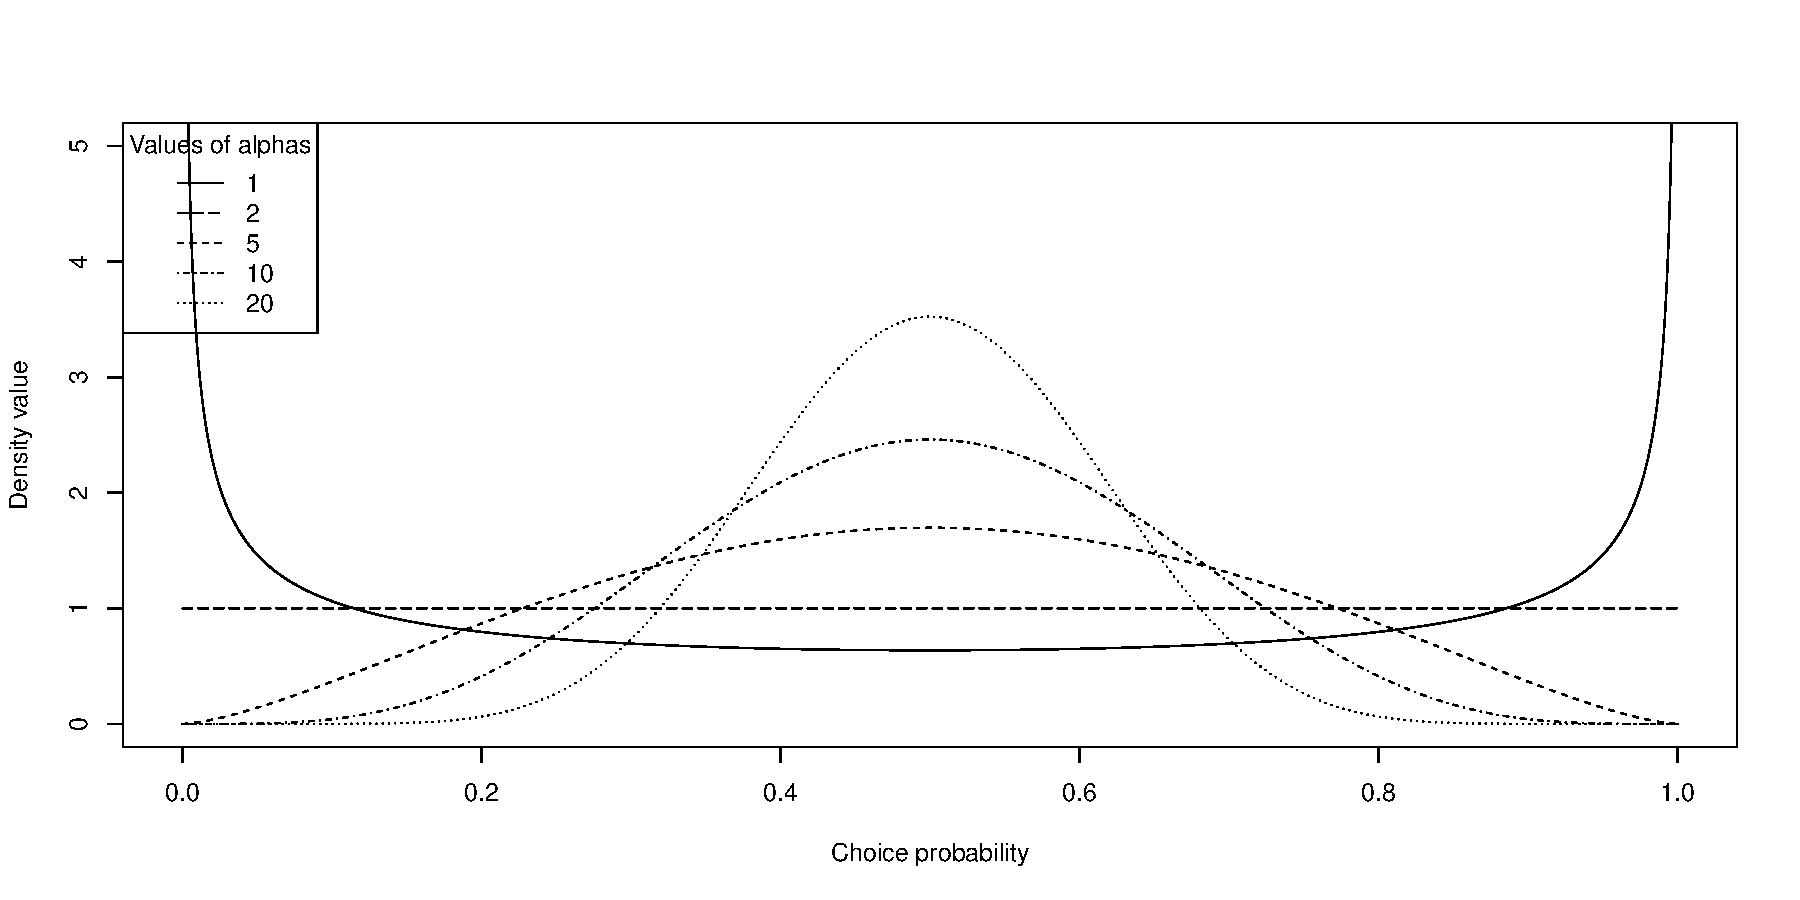
\includegraphics[width=15cm]{Figures/bcp.pdf}
	\caption{Density of binary choice probabilities for $\alpha = 1, 2, 5, 10, 20$}\label{f:bcp}
	\end{center}
\end{figure}

The parameter $\lambda$ describes the degree of dependence of choice probabilities across \menus{}.
For $\lambda = 0$, the choice probability vectors $P_A(\cdot)$ are mutually independent, across $A \subseteq T$.
For $\lambda = 1$, the random choice structure satisfies random utility with probability one.
For $\lambda = 1$, and only this value, the prior does not have full support on $\Delta$.
Details on the prior distributions for $P$, including some of its desirable properties, are given in \citeasnoun{McCaMarl13}.

It remains to specify the unknown parameters $\alpha$ and $\lambda$.
One can choose fixed values, but a more flexible approach allows for learning about plausible values of $\alpha$ and $\lambda$ through data.
In this approach, one provides a prior distribution for $\alpha$ and $\lambda$, completing a hierarchical prior for $P$.
Just as $P$ can be marginalized out to obtain the marginal density $f_M({\bf x})$ when using a non-hierarchical prior density $f_M(P)$ for $P$, we can marginalize out $\alpha$, $\lambda$ and $P$ using a hierarchical prior consisting of a prior density $f_M(\alpha,\lambda)$ for $\alpha$ and $\lambda$ and the density $f(P|\alpha,\lambda)$ in \citeasnoun{McCaMarl13}.
The result is the marginal density
\[
  f_M({\bf x}) = \int f({\bf x}|P) f(P|\alpha,\lambda) f_M(\alpha,\lambda) \, dP\, d\alpha\, d\lambda.
\]
Again, the marginal likelihood $f_M({\bf x}_{\mathrm{obs}})$ is obtained by evaluating this at the observed choice dataset ${\bf x}_{\mathrm{obs}}$.

Following \citeasnoun{McCaMarl14} and \citeasnoun{McCaStobMarlParkBrow20}, we specify an encompassing model using a hierarchical prior distribution for $P$ consisting of the prior density $f(P|\alpha,\lambda)$ and a prior distribution of $(\alpha,\lambda)$ where $\alpha$ and $\lambda$ are {\em a priori} independent, $\alpha$ has a Gamma distribution with shape parameter $a_1 + a_2$ and rate parameter $b$, $\lambda$ has a Beta distribution with shape parameters $a_1$ and $a_2$.
Like those papers, we use various choices of the hyper-parameter vector $(a_1,a_2,b)$, to illustrate the sensitivity of results to the choice of encompassing model.
However, the particular choices of $(a_1,a_2,b)$ we use here are different.
In part, this is because the present paper is concerned with population, rather than individual choice.
Anticipating some heterogeneity across individuals, we shift prior weight towards higher values of $\alpha$, and therefore away from choice probabilities close to zero or one.
Also, we learned from the analysis of these previous experiments that results were fairly insensitive to the prior for $\alpha$, and that values of $\lambda$ close to one were strongly favoured.
Accordingly, we use the same prior for $\alpha$ for each encompassing model and put more prior weight on values of $\lambda$ closer to one than in \citeasnoun{McCaMarl14} and \citeasnoun{McCaStobMarlParkBrow20}.

Table \ref{t:hyper} shows the values of $(a_1, a_2, b)$ for four encompassing models used in the empirical analysis.
Model $M_{\mathrm{ind}}$ features a degenerate distribution for $\lambda$, with all prior mass at the value $\lambda = 0$, which makes the $P_A(\cdot)$ {\em a priori} independent.
We will use this model only for testing the less restrictive axioms (WST, MST, TI) as the prior probability of the other axioms under $M_{\mathrm{ind}}$ is too low to measure easily.
The encompassing models $M_1$, $M_2$ and $M_3$ feature dependence of $P_A(\cdot)$ across $A$ and are suitable for testing strong stochastic transitivity and the multiple choice axioms.

Table \ref{t:hyper} also indicates the prior mean, variance and standard deviation of $\alpha$ and $\lambda$ for the four encompassing models.
As we go from model $M_1$ to $M_2$ and then $M_3$, the prior distribution of $\lambda$ concentrates more and more probability mass near $\lambda = 1$.

\begin{table}
\begin{center}
\begin{tabular}{cccccccccc}
 & $a_1$ & $a_2$ & b &
 $E[\alpha]$ & $\mathrm{Var}[\alpha]$ & $\sigma_\alpha$ & $E[\lambda]$ & $\mathrm{Var}[\lambda]$ & $\sigma_\lambda$ \\
 \hline
 $M_{\mathrm{ind}}$ & 0.00 & 3.00 & 3.00 & 9.00 & 27.00 & 5.196 & 0 & 0 & 0 \\
 \hline
 %$M_0$ & 2.00 & 0.25 & 4.00 & 9.00 & 36.00 & 6.000 & 0.889 & 0.030 & 0.174 \\
 $M_1$ & 2.00 & 1.00 & 3.00 & 9.00 & 27.00 & 5.196 & 0.667 & 0.0556 & 0.236 \\
 $M_2$ & 2.50 & 0.50 & 3.00 & 9.00 & 27.00 & 5.196 & 0.883 & 0.0347 & 0.186 \\
 $M_3$ & 2.75 & 0.25 & 3.00 & 9.00 & 27.00 & 5.196 & 0.917 & 0.0191 & 0.138 \\
 \hline
\end{tabular}
\end{center}\caption{Prior hyper-parameters and moments for various encompassing models}\label{t:hyper}
\end{table}

\section{Inferential Methods}\label{s:inference}

For any given choice dataset, our principal inferential objective is to test various axioms of discrete choice, using Bayes factors comparing models constrained by axioms to encompassing models.
A secondary inferential objective, not pursued extensively here, is to describe the posterior distribution of $P$ and the parameters $\alpha$ and $\lambda$ of the encompassing or the constrained models.
Both inferential exercises are based on posterior simulation methods outlined in \citeasnoun{McCaMarl14}.

The posterior distribution $\alpha,\lambda,P|{\bf x}_\mathrm{opt}$, represents what we learn, relative to the prior distribution of $\alpha$, $\lambda$ and $P$, from the choice dataset ${\bf x}_\mathrm{opt}$.
The posterior distribution is analytically intractable and we use Markov chain Monte Carlo (MCMC) methods to obtain a large posterior sample targeting the posterior distribution.
The posterior sample does not consist of independent draws, but there are standard methods for quantifying simulation error; that is, the difference between posterior sample moments and their population counterparts.
We use the overlapping batch means (OBM) method, whose properties are described in \citeasnoun{FlegJone10}, to compute the numerical standard error of posterior sample means.

We compute Bayes factors for all model comparisons.
Suppose we are comparing any two Bayesian discrete choice models $M$ and $M'$, and we observe a choice dataset ${\bf x}$.
Then the posterior odds ratio giving the relative posterior probabilities of $M$ and $M'$ can be expressed as
\[
  \frac{\Pr[M|{\bf x}_\mathrm{opt}]}{\Pr[M'|{\bf x}_\mathrm{opt}]} = \frac{\Pr[M]}{\Pr[M']}
  \cdot
  \frac{f_{M}({\bf x}_\mathrm{opt})}{f_{M'}({\bf x}_\mathrm{opt})}
  %\frac{\Pr[{\bf x}|M]}{\Pr[{\bf x}|M']}
\]
This result follows easily from Bayes' rule and does not depend on how many models are under consideration.
The expression on the right hand side is the product of two factors.
The first is the prior odds ratio and the second is a ratio of marginal likelihoods called the {\em Bayes factor}---see \citeasnoun{Berg85} or \citeasnoun{BernSmit94}.
The marginal likelihoods $f_{M}({\bf x}_\mathrm{opt})$ and $f_{M'}({\bf x}_\mathrm{opt})$ are the probabilities of observing the choice data ${\bf x}_\mathrm{opt}$ if the models $M$ and $M'$ (respectively) are true.
The ratio measures the relative out-of-sample predictive performance of the two models, with a value greater t{}han one favouring model $M$.

In the special case where the denominator model is an encompassing model $M_e$ and the numerator model is the constrained model $M_c$ obtained by truncating the density $f_{M_e}(P)$ associated with $M_e$ to the region $\Lambda$ defining an axiom, then the Bayes factor becomes
\begin{equation}\label{e:BF}
  \frac{f_{M_c}({\bf x}_\mathrm{opt})}{f_{M_e}({\bf x}_\mathrm{opt})} =
  \frac{\Pr_{M_e}[{\bf X} = {\bf x}_\mathrm{opt}|P \in \Lambda]}{\Pr_{M_e}[{\bf X} = {\bf x}_\mathrm{opt}]} = \frac{\Pr_{M_e}[P \in \Lambda|{\bf X} = {\bf x}_\mathrm{opt}]}{\Pr_{M_e}[P \in \Lambda]}.
\end{equation}

The second equation of \eqref{e:BF} follows from Bayes' rule; see \citeasnoun{KlugHoij07}; the far right hand side of \eqref{e:BF} is the ratio of posterior to prior probability of the axiom holding according to the encompassing model.{}
A large numerator indicates an axiom that is highly probable in light of the data; a small denominator indicates that an axiom is restrictive.
This ratio also suggests a practical way of computing approximations of Bayes factors: since the probability of an event is just the expectation of an indicator function for the event, we can approximate numerator and denominator using Monte Carlo methods.

We compute prior and posterior probabilities of axioms numerically using the simulation methods described in \citeasnoun{McCaMarl14}.
We compute numerical standard errors of prior and posterior probabilities using the OBM method and combine these standard errors to compute standard errors for Bayes factors using the delta method, introduced in \citeasnoun{Kell28}.

\section{Experimental Design}\label{s:design}

The experiment consisted of an internet survey conducted between August 10, 2017 and August 31, 2017.
A total of 1042 participants completed the survey.

Participants were recruited by Survey Sampling International (SSI) from their Canadian panel, designed to be representative of the Canadian adult population.
According to the SSI Global Panel Book 2017, included in the experimental supplement to this paper, the Canadian panel consists of 577,356 members.
SSI screens potential members for reliability and requires that all participants be at least 18 years of age.
They also carefully verify the identity of their participants for each survey.
The Canadian panel is 42\% male and 58\% female and has the following age distribution: the percentage of members in the age range 18-24 is 36\%; 25-34, 25\%; 35-54, 26\%; 55 and older, 13\%.
Compensation of participants includes cash and other rewards.
The experimental supplement to this paper describes in more detail the recruitment and compensation procedures followed by SSI, although some of the information about these procedures is proprietary.

We chose not to impose any additional restrictions on our sample of participants.
However, since invited participants must complete the survey to be included in the sample, there is some self-selection.
We have full information on age, province and sex for all 1042 participants in our sample.
There are 515 men (49.4\%) and 527 women (50.6\%).
Age ranges from 18 to 88; the percentage of participants in the age bracket 18-24 is 11.4\%; 25-34, 17.8\%; 35-54, 38.3\%, 55 and older, 32.5\%.
% quartiles of age were 32, 46 and 58.
The number of participants in Alberta was 124; British Columbia, 136; Manitoba, 36; New Brunswick, 23; Newfoundland and Labrador, 16; Northwest Territories, 1; Nova Scotia, 29; Ontario, 391; Prince Edward Island, 4; Quebec, 251; Saskatchewan, 30; and Yukon, 1.
Participants could take as long as they liked to complete the survey.
The quartiles of total duration were 7.1, 10.0 and 13.9 minutes.
Three participants took longer than 24 hours, and the shortest duration was 1.7 minutes.
Participants were given the opportunity to leave written feedback on the experiment upon completion.

Programming and hosting of the survey were provided by the Institute for Choice at the University of South Australia.

Our experiment features $J=32$ choice domains, including fine art, travel itineraries and pizza toppings.
Each domain consists of a universe of five related choice objects.
The names of the choice domains are shown in Table \ref{t:domains}, together with the question (or an excerpt of the question, with excluded text indicated by an ellipsis) used to elicit a response from the participant.
Appendix \ref{s:domains} describes each domain in detail, including the question, the five choice objects and, where applicable, a source for the information used to construct the question.
Figure \ref{f:screenshots} shows screenshots for the ``Travel'' and ``Coffee'' domains.
There are $I=2^{5}-5-1=26$ \menus{} (binary and larger subsets of the five-element universe) for each domain, for a total of $JI=910$ \menus{}.
The screenshot for the ``Travel'' domain in Figure \ref{f:screenshots} shows a menu with two of the five choice objects in that domain; the ``Coffee'' screenshot, four of the five choice objects in the ``Coffee'' domain.

\begin{table}[h!]
  \begin{center}
    \caption{Choice domains of the experiment}
    \label{t:domains}
    \begin{small}
    \begin{tabular}{lp{12cm}}
      Domain name & Question\\
      \hline
      	Male stars & Which movie star would you choose to have lunch with? \\
		Female stars & Which movie star would you choose to have lunch with? \\
		Films & Judging from the following descriptions of films, which one of the films would you choose to see? \\
		Star pairs & Knowing only who is starring, which one of these new films would you choose to see? \\
		Pizzas & Which one of the following pizzas would you choose? \\
		Juices & Which one of the following fresh juices would you choose? \\
		Colours & Which one of the following colours do you like best? \\
		Colour Pairs & Which one of these colour combinations do you like best? \\
		Events & Which one of the following events do you think is most likely to happen in the next twenty years? \\
		Radio formats & Suppose you were on a two hour road trip and you have a choice among radio stations with the following formats.
Which one would you choose? \\
		Music & Which one of the following musical artists do you like the best? \\
		Aborig. art & Which one of the following examples of Australian aboriginal art do you like the best? \\
		Impress. art & Which one of the following examples of Impressionist art do you like the best? \\
		Sentences & Which one of the following sentences do you find the most grammatically acceptable? \\
		Travel & Which one of the following travel destinations would you most like to visit? \\
		Marijuana & Which one of the following marijuana policies would you choose? \\
		Latitude & Which one of the following cities do you think is furthest north? \\
		Dots & Which one of the following boxes do you think has the greatest number of points? \\
		Triangles & Which one of the following triangles do you think has the greatest area? \\
		Population & Which one of the following countries do you think has the largest population? \\
		Area & Which one of the following countries do you think has the greatest surface area, including inland bodies of water? \\
		Beer & ... Given that you had to choose one brand to buy on this information alone, which one would you choose? \\
		Cars & Which one of the following cars would you choose to drive, all other features
begin equal? ... \\
		Restaurants & Which one of the following restaurants would you choose for your next restaurant meal...? \\
		Itineraries I & Which one of the following flight itineraries would you choose? ... \\
		Payoffs & Which one of the following would you choose? \\
		Phone plans & Of the following cell phone plans, which one would you choose? ... \\
		Hotel rooms & ... Which one of the following hotels would you choose, ...? \\
		Itineraries II & Which one of the following flight itineraries would you choose? ... \\
		Televisions & Which one of the following televisions would you choose to buy ...? \\
		Coffee & Which one of the following ground coffees would you choose? \\
		Charity & Suppose someone was donating a total of 100 dollars to a combination of charities,
on your behalf.
Which one of the following divisions of the 100 dollars would you choose? \\
    \end{tabular}
    \end{small}
  \end{center}
\end{table}

Regarding the assignment of participants to \menus{}, our intended design was as follows.
Within each domain, each of the $I$ \menus{} is presented exactly $N=40$ times, once to each of $N$ distinct participants.
Each participant faces exactly one \menu{} from each domain, for a total of $J$ trials.
Thus the total number of participants is $NI=1040$, and the total number of trials is $NIJ=33,280$.
For each domain $j$, the $NI$ participants are randomly partitioned into $I$ groups of size $N$, with participants in each group seeing the same \menu{} from that domain.
Random partitions are uniformly distributed and mutually independent across domains.
Elements of a \menu{} are presented in random position (left, middle, right, for example) on the screen, independently across the $N$ participants facing that \menu{}.
The $J$ trials assigned to each participant are presented in random order, independently across participants.
Random partitions, positions and trial order are mutually independent.

In the event, two extra participants completed the experiment, and their choices were included in the analysis.
For each domain, two \menus{} were presented 41 times instead of 40 and the total number of trials is 33,344.

Participants choose exactly one object from each \menu{}.
For some domains, participants select radio buttons and in others, they select pictures, which are then identified by a border.
Figure \ref{f:screenshots} shows one screenshot for each kind of domain.
In each case, participants can modify their choice before they confirm it by clicking on a button labelled ``$>>$''; once they click this button, they cannot go back and change their response.
A progress bar indicates progress through the experiment.

\begin{figure}
	\begin{center}
	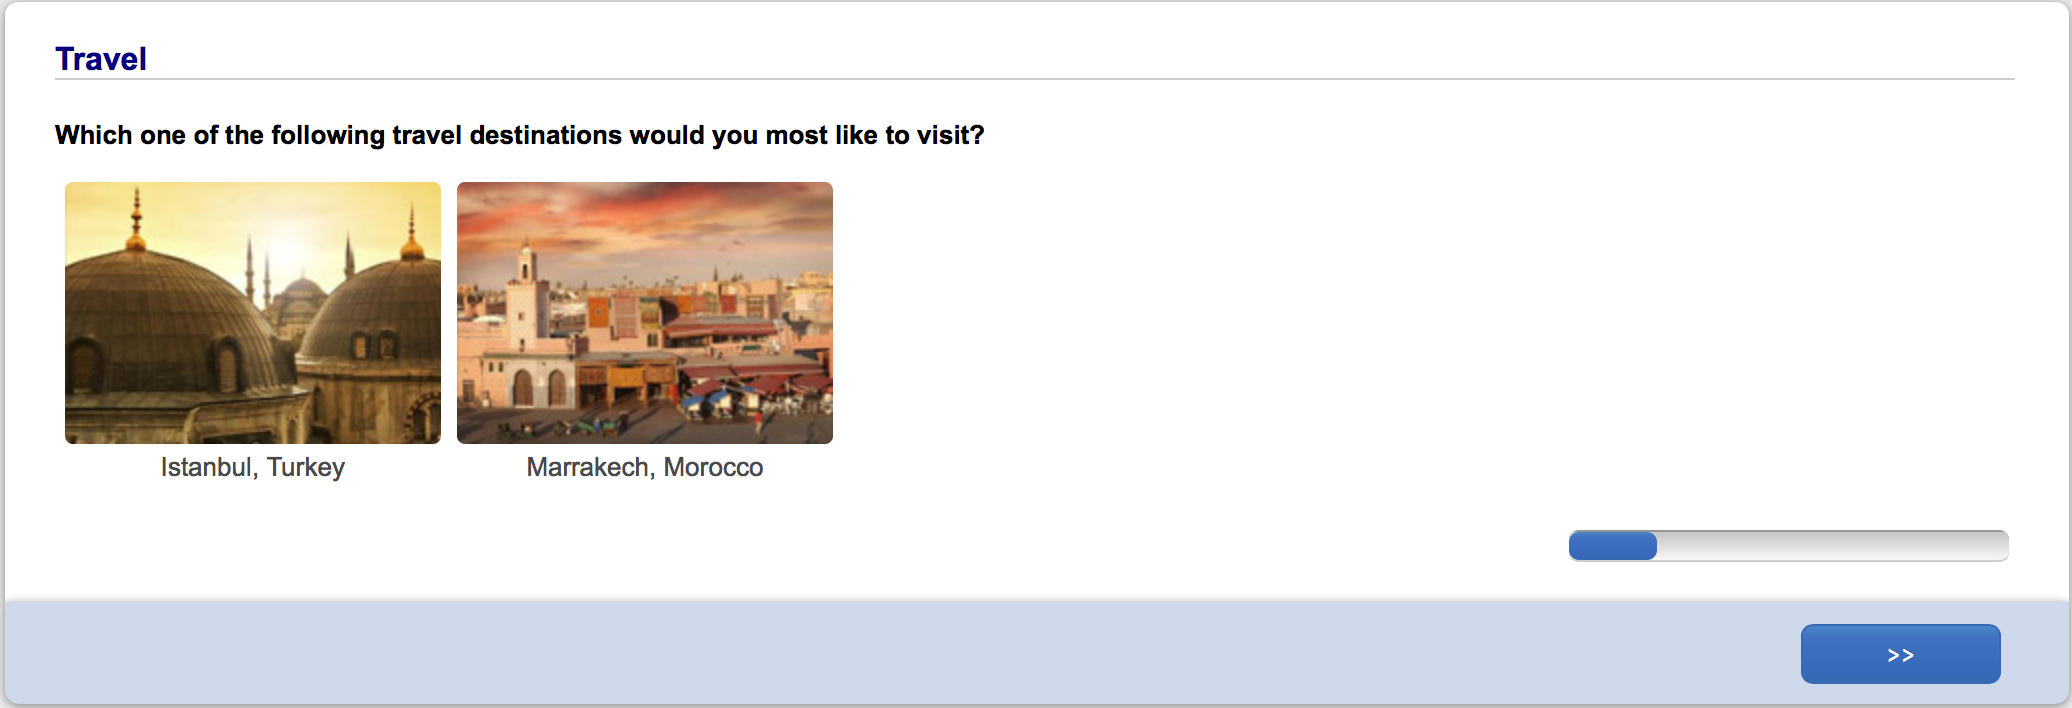
\includegraphics[width=15cm]{Population_study_design/screenshot_Travel.png}
	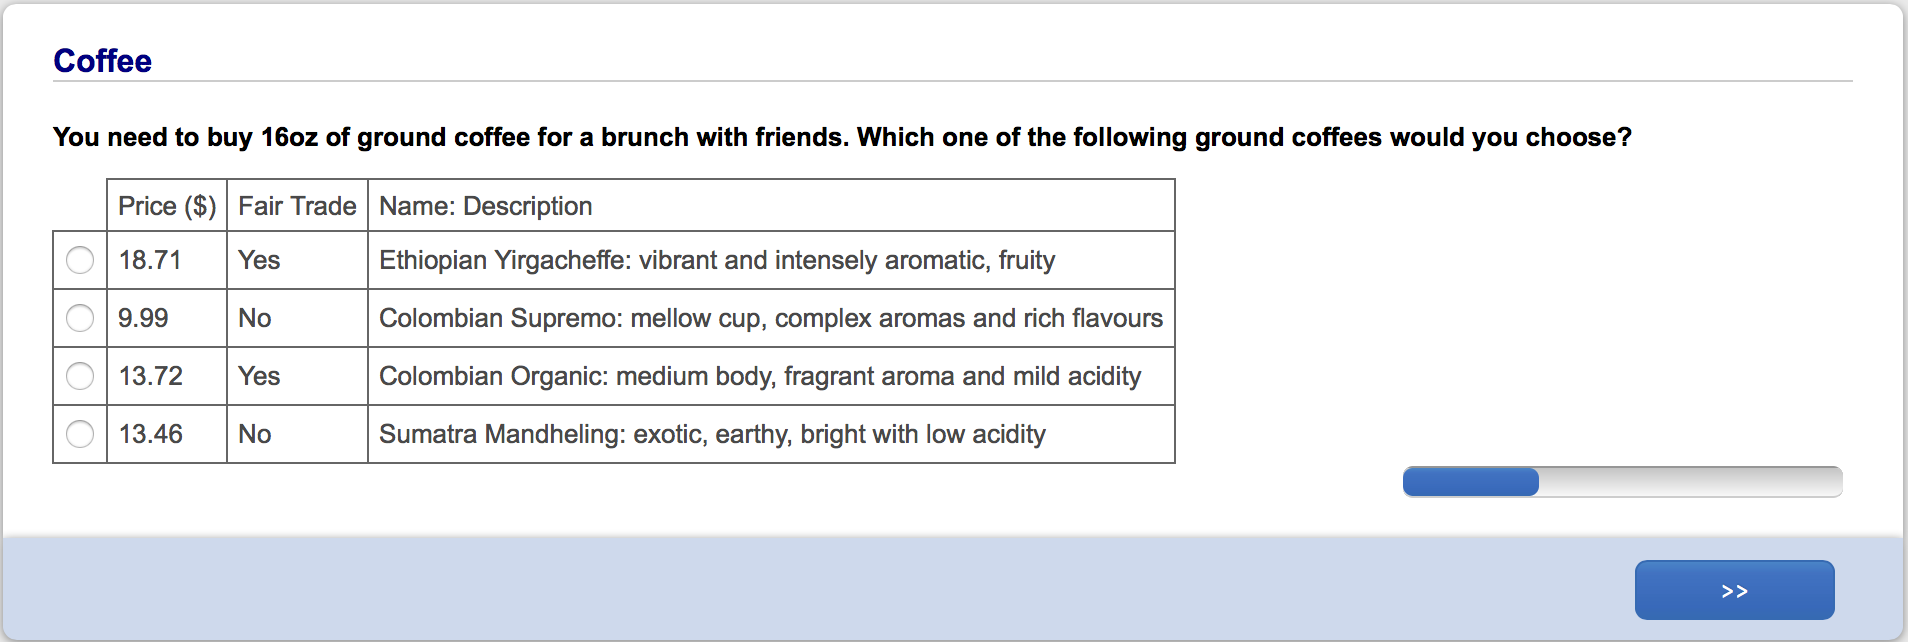
\includegraphics[width=15cm]{Population_study_design/screenshot_Coffee.png}
	\caption{A screenshot for the ``Travel'' domain, in which participants select pictures, and a screenshot for the ``Coffee'' domain, in which participants select radio buttons. In the experiment and in electronic versions of this paper, these photographs are in colour.}\label{f:screenshots}
	\end{center}
\end{figure}

\section{Results}\label{s:results}

We begin by providing some evidence that participants were engaged in the experiment.
We then show some data summaries for one of the experimental domains, for illustrative purposes.
The supplement to the paper provides the same data summary for the other domains.
We then report Bayes factors in favour of constrained models against encompassing models, for several choices of constraining axiom and encompassing model.
Finally, we report posterior quantiles of $\alpha$ and $\lambda$ for the various choice domains.

\subsection{Engagement of participants}

Evidence for a high level of engagement on the part of participants comes from written feedback, timing information, and the responses to questions where the objectively ``correct'' answer is known to most people.
Most of the feedback left by participants was positive and many indicated a high level of interest.
All feedback from participants is available in the experimental supplement.
The median participant took $18.75s$ per domain; three quarters of them took longer than $13.31s$ per domain.
The domain ``Latitude'', where participants are prompted with the question ``Which one of the following cities do you think is furthest north'' is one of the domains whose elements have an objective order.
In this domain, there are two pairs of cities where the objective order of latitude should be familiar to most people: one is ``London, United Kingdom'' and ``Paris, France''; the other is ``Vancouver, Canada'' and ``Seattle, United States''.
We would expect most attentive participants to choose the city that is actually furthest north.
Indeed, of the 40 participants offered the binary choice between London and Paris, 32 chose London and of the 40 participants offered the binary choice between Vancouver and Seattle, 36 chose Vancouver.
Recall that the participants are residents of Canada.

\subsection{Observed binary and ternary choice frequencies}

Figure \ref{f:colours} illustrates all binary and ternary choice frequencies for the ``Colours'' domain, where the prompt is ``Which one of the following colours do you like best?'' and the universe of objects is $\{a,b,c,d,e\}$ where $a$ is Red, $b$ is Purple, $c$ is Pink, $d$ is Blue and $e$ is Green.
It also shows how these frequencies relate to regularity and the multiplicative inequality.
Similar figures, as well as raw data, for all 32 choice domains can be found in the supplement to the paper.

The figure consists of 10 panels.
Each panel corresponds to one of the ten tripleton \menus{} from that domain, and features an equilateral triangle, with vertices labelled with the three choice objects in that \menu{}.
Take the first panel as an example, where the corresponding \menu{} is $A \equiv \{a,b,c\}$ and the vertices are labelled $a$ (bottom left), $b$ (top) and $c$ (bottom right) accordingly.
Each point in the interior or on the boundary of the triangle represents a triple $(P_A(a),P_A(b),P_A(c))$ of choice probabilities, in a Barycentric coordinate system.
Thus, if triangle $abc$ has unit height, the distance of a point to the right side of the triangle is $P_A(a)$, the distance to the base is $P_A(b)$ and the distance to the left side is $P_A(c)$.
The point is also the convex combination of the vertices $a$, $b$ and $c$---which have Barycentric coordinates $(1,0,0)$, $(0,1,0)$ and $(0,0,1)$, respectively---with weights $P_A(a)$, $P_A(b)$ and $P_A(c)$.
The solid point in the interior of the triangle gives the triple $(\hat P_A(a), \hat P_A(b), \hat P_A(c))$ of choice frequencies observed for menu $A$ of this domain, the sample counterpart of the ternary choice probability vector $(P_A(a),P_A(b),P_A(c))$.

The hollow dots on the left, right and bottom sides of the triangle represent binary choice frequencies $\hat p(a,b)$, $\hat p(b,c)$ and $\hat p(a,c)$, sample counterparts to the probabilities $p(a,b)$, $p(b,c)$ and $p(a,c)$, respectively.
For example, the dot on the left side of the triangle is the convex combination of the vertices labelled $a$ and $b$, with weights $\hat p(a,b)$ and $\hat p(b,a)$ respectively.

The downward pointing (blue in electronic versions of this paper) triangle in each figure gives necessary conditions on the ternary choice frequencies, given the three binary choice frequencies, for regularity to hold for choice frequencies on the sub-universe $T' \equiv \{a,b,c\}$: ternary probabilities within the blue triangle satisfy $P_A(a) \leq \min(\hat p(a,b), \hat p(a,c))$, $P_A(b) \leq \min(\hat p(b,a), \hat p(b,c))$ and $P_A(c) \leq \min(\hat p(c,a), \hat p(c,b))$.
Similarly, the small upward pointing (red) triangle gives necessary conditions on the ternary choice frequencies, given the three binary choice frequencies, for the multiplicative inequality to hold for choice frequencies on $T'$: ternary probabilities in the red triangle satisfy $P_A(a) \geq \hat p(a,b) \hat p(a,c)$, $P_A(b) \geq \hat p(b,a) \hat p(b,c)$ and $P_A(c) \geq \hat p(c,a), \hat p(c,b)$.

\begin{figure}
	\caption{Binary and ternary choice frequencies for the Colours domain, where the prompt is ``Which one of the following colours do you like best?'' and the universe of objects is $\{a,b,c,d,e\}$, where $a$ is Red, $b$ is Purple, $c$ is Pink, $d$ is Blue and $e$ is Green.}\label{f:colours}
	\centering
	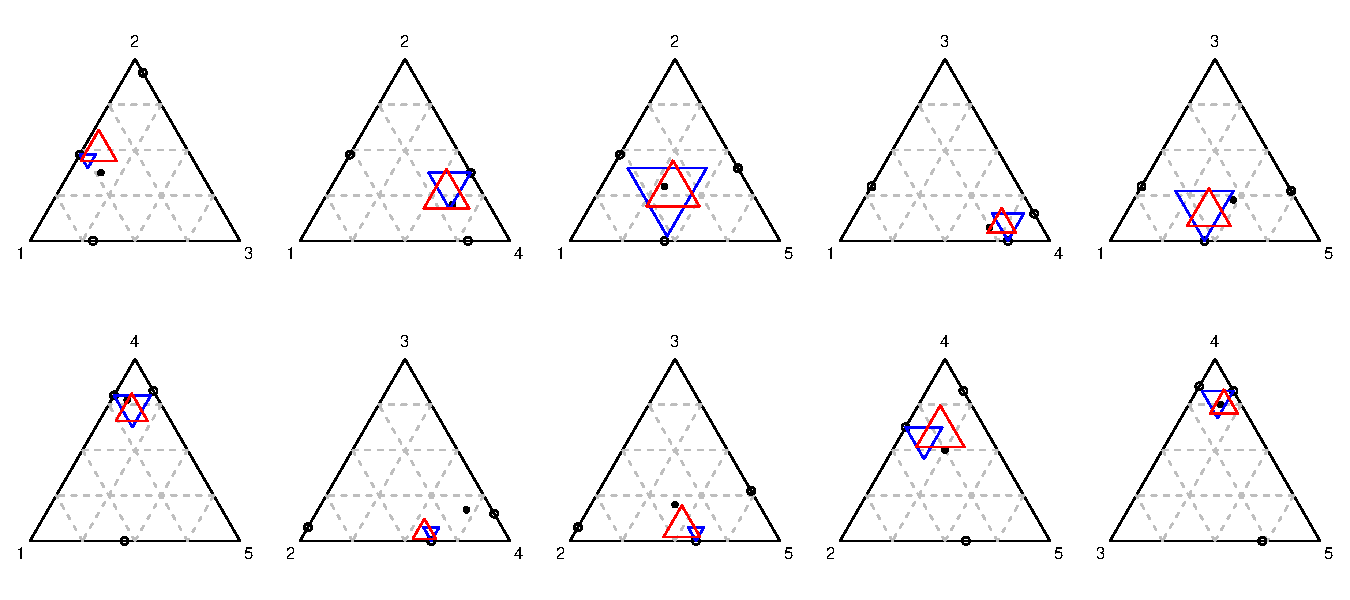
\includegraphics[width=16cm]{./Population_study_data/Simplexes/Colours.pdf}
\end{figure}

\subsection{Tests of axioms using Bayes factors}

For each choice domain, we computed log Bayes factors in favour of several models, all relative to the encompassing model $M_3$, which was favoured over $M_1$ and $M_2$ for 31 out of the 32 domains.
We did this for the three encompassing models and for the constrained models defined by all possible pairs of encompassing model and axiom.

Figure \ref{f:binary_BF} gives, for each domain, log Bayes factors for various combinations of binary choice axiom and encompassing model, relative to encompassing model $M_3$.
There is a panel for each domain, with three columns of points, corresponding to the three encompassing models $M_1$, $M_2$ and $M_3$.
In each column, the circle gives the log Bayes factor of the corresponding encompassing model against $M_3$; in the third column, this value is always zero, since the log Bayes factor of any model relative to itself is zero.
The triangle, square and cross give log Bayes factors of the constrained model consisting of the restriction of the corresponding encompassing model to the regions $\Lambda_{\mathrm{WST}}$, $\Lambda_{\mathrm{MST}}$ and $\Lambda_{\mathrm{SST}}$, respectively.
(Results for the remaining binary choice axiom, the triangle inequality, are reported below.)
For the Charity choice domain, the posterior probability of SST is close to zero for all three encompassing models; while this makes numerical estimation of the log Bayes factor in favor of SST difficult, we can conclude that the evidence against SST is very strong\footnote{\citeasnoun{KassRaft95} classify log Bayes factors between 0 and 1 as ``not worth more than a bare mention'', those between 1 and 3 as providing ``positive evidence'', those between 3 and 5 as providing ``strong evidence'' and those above 5 as providing ``very strong evidence''. We will adopt these categories, but refer to the first two as giving ``weak'' evidence and ``moderate'' evidence.} for this choice domain.

Across domains, the support for these binary choice axioms varies.
With the exception of SST for a few domains (Male stars, Pizzas, Radio formats, Travel, Area and Charity) the evidence is moderate at best.
For these few domains, the evidence is much stronger; interestingly, the evidence is sometimes in favour of SST and sometimes against.
For most domains, the evidence for these stochastic transitivity axioms is monotonic, in the sense that log Bayes factors are increasing or decreasing as we go from no axiom (none) to WST to MST to SST.
A clear exception is the ``Latitude'' domain, where in decreasing order of Bayes factor, we have MST, then WST, then none then SST.
In most domains, the order of log Bayes factors, and to some extent the differences, are robust to the encompassing model.
For the exceptions, such as the Events domain, the differences are small and therefore there is little evidence supporting any one of these axioms over the others.

\begin{figure}
	\begin{center}
	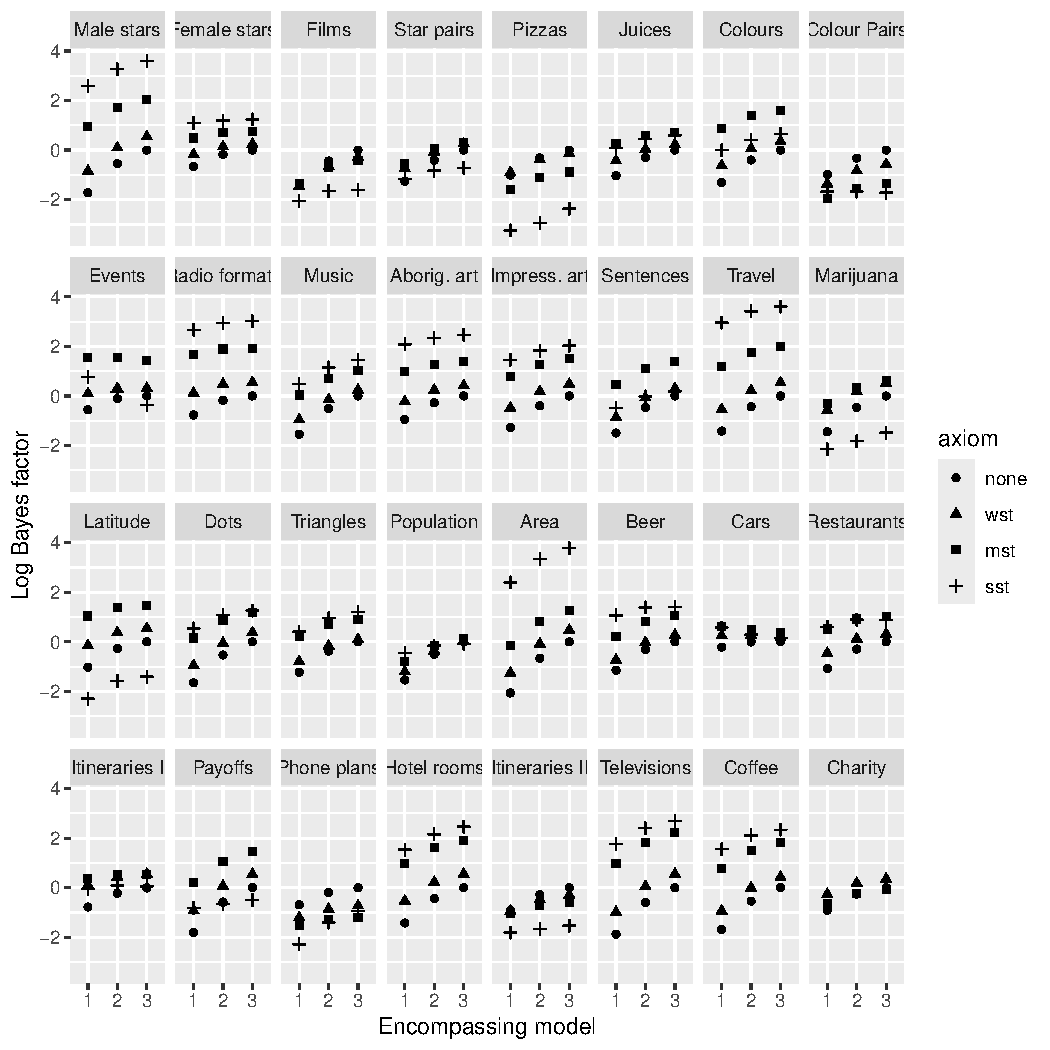
\includegraphics[width=16cm]{Figures/binary_BF}
	\caption{Log Bayes factors for 32 domains, by encompassing model and binary choice axiom. All log Bayes factors are relative to encompassing model $M_3$. The ``encompassing model'' indices 1, 2 and 3 correpond to models $M_1$, $M_2$ and $M_3$.}\label{f:binary_BF}
	\end{center}
\end{figure}

Figure \ref{f:multiple_BF} gives, for each choice domain, log Bayes factors for various combinations of multiple choice axiom and encompassing model, relative to encompassing model $M_3$.
It is organized in the same way as Figure \ref{f:binary_BF}.
For the multiplicative inequality, the posterior probability is close to zero for the choice domains ``Latitude'', ``Itineraries I'' and ``Payoffs'', whatever the encompassing model, implying a strong rejection of that axiom.
Evidence for the multiplicative inequality varies a lot across choice domain, from moderate evidence in favour to very strong evidence against.
The evidence is fairly robust to the choice of encompassing model.
For regularity and random utility, the evidence is weaker, but more consistent across choice domains.
In most cases, the log Bayes factors either favour random utility and regularity over the encompassing models, or are very close to zero, representing little evidence either way.
Across domains and encompassing models, the evidence in favour of random utility is very similar to the evidence in favour of regularity, which is a necessary condition for random utility.
In most cases, the evidence in favour of regularity is greater than that in favour of random utility, indicating some evidence against the higher order features of random utility, but this evidence is quite weak.
For individual domains, the evidence in favour of random utility and regularity are at best slight, but collectively, the evidence is much stronger: the log Bayes factor in favour of regularity holding jointly across domains is the sum over domains of the log Bayes factors in favour of regularity, and likewise for random utility.
In both Figures \ref{f:binary_BF} and \ref{f:multiple_BF}, the variation in predictive performance of an axiom across underlying encompassing model is much less than the variation in that across the encompassing models themselves.
This suggests similar implications for observables between imposing the axiom and increasing the prior dependence of $P_A(\cdot)$ across \menus{} $A$, as measured by $\lambda$.

\begin{figure}
	\begin{center}
	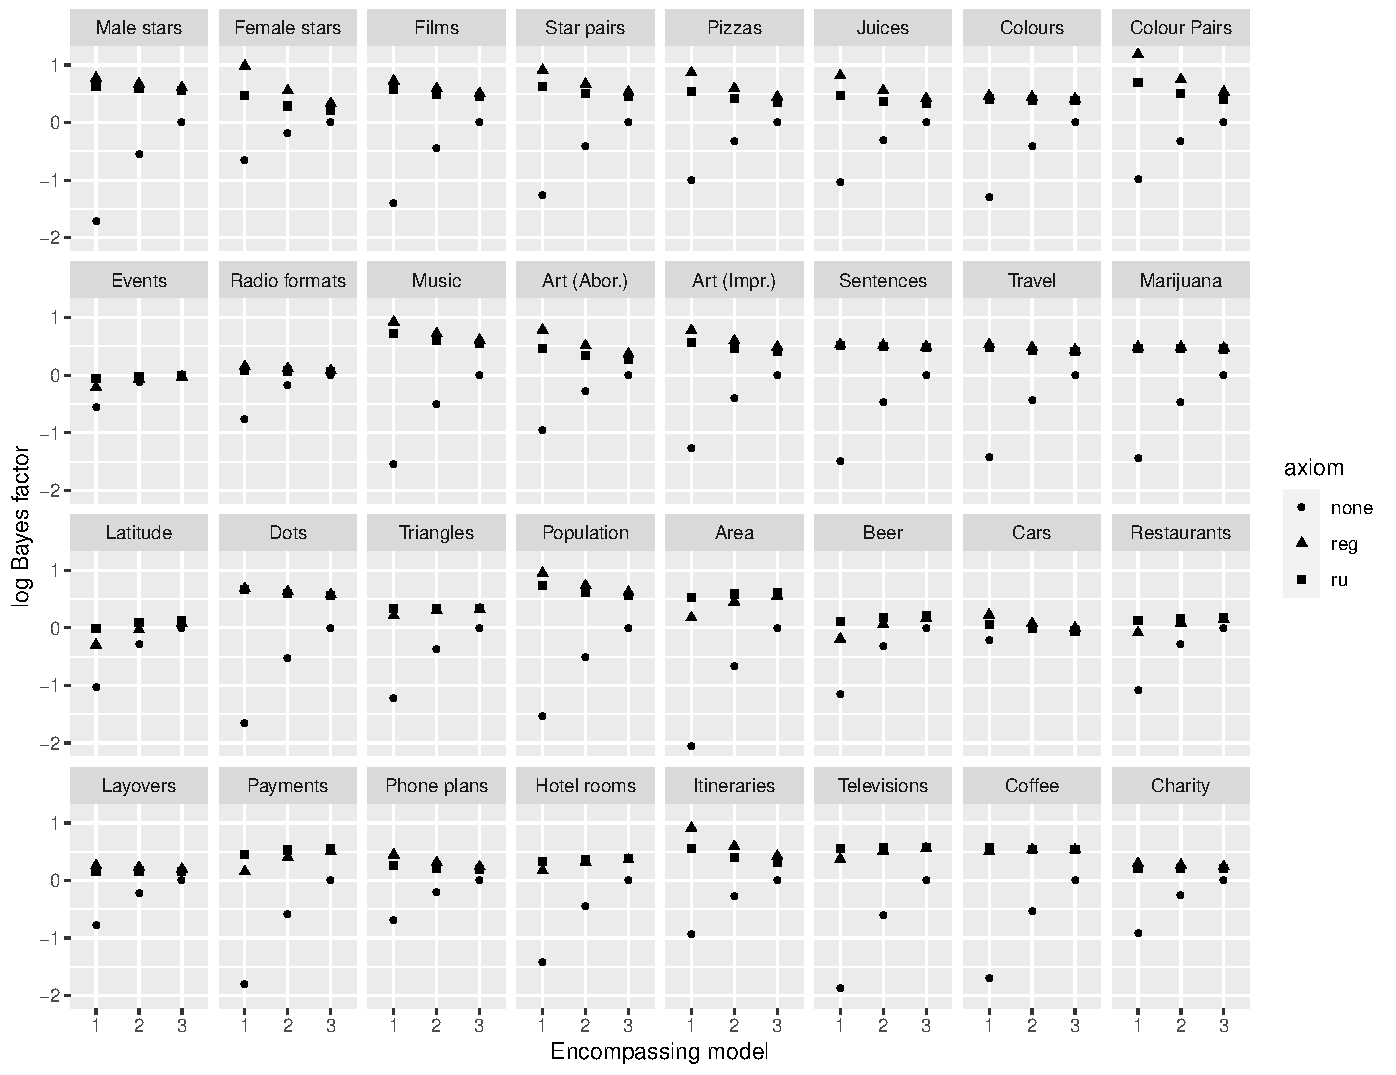
\includegraphics[width=16cm]{Figures/multiple_BF}
	\caption{Log Bayes factors for 32 domains, by encompassing model and multiple choice axiom. All log Bayes factors are relative to encompassing model $M_3$. The ``encompassing model'' indices 1, 2 and 3 correspond to models $M_1$, $M_2$ and $M_3$.}\label{f:multiple_BF}
	\end{center}
\end{figure}

Table \ref{t:bin} shows Bayes factors in favour of WST, MST and TI against the encompassing model $M_{\mathrm{ind}}$, where $\lambda = 0$ and choice probabilities $P_A(\cdot)$ are thus independent across \menus{}.
For comparison, it also shows Bayes factors in favour of these axioms against $M_3$, the most favoured encompassing model for all domains except one.
For encompassing model $M_{\mathrm{ind}}$, the evidence favours WST, as it does for $M_3$.
However, the evidence is stronger, due to the relatively lower prior probability of WST when the $P_A(\cdot)$ are independent.
The two models mostly agree on whether MST is favoured or not.
Again, the evidence is stronger for $M_{\mathrm{ind}}$, and is either moderate or strong for most domains.
Even in the four domains where the evidence is against MST, this evidence is weak.

For both encompassing models, the Bayes factor in favour of TI varies little across domain.
This is because for most domains, the posterior probability of TI is close to one and so the log Bayes factor in favour of TI is close to its upper bound, which is equal to minus the logarithm of the prior probability of TI.
The high prior probability of TI, especially for $M_3$, limits the amount of evidence that the data can provide in favour of TI.
Even the uniformly high posterior probability of TI across domains is less revealing than it may appear, in light of two observations.
First, for any given choice domain, binary choice frequencies will tend to be more moderate for populations than for individuals, due to aggregation over heterogeneous individuals.
Second, when binary choice probabilities are moderate, the triangle inequality is much less limiting.
In fact, the triangle inequality holds for any RCS where all binary choice probabilities lie in the interval $[\tfrac{1}{3},\tfrac{2}{3}]$.
It is not very surprising then, that in this population choice experiment, binary choice frequencies tend to be more moderate than those in individual choice experiments, and that the posterior probability of the triangle inequality is very close to one.

\begin{table}
  
\begin{tabular}[t]{lrrrrrr}
\toprule
\multicolumn{1}{c}{ } & \multicolumn{3}{c}{Model $M_{\mathrm{ind}}$} & \multicolumn{3}{c}{Model $M_3$} \\
\cmidrule(l{3pt}r{3pt}){2-4} \cmidrule(l{3pt}r{3pt}){5-7}
Domain & WST & MST & TI & WST & MST & TI\\
\midrule
Male stars & 1.67 & 3.76 & 0.70 & 0.54 & 2.05 & 0.062\\
Female stars & 1.03 & 1.75 & 0.71 & 0.24 & 0.75 & 0.062\\
Films & 0.18 & -0.43 & 0.50 & -0.29 & -0.41 & 0.061\\
Star pairs & 0.54 & 0.42 & 0.70 & 0.25 & 0.32 & 0.062\\
Pizzas & 0.21 & -0.97 & 0.69 & -0.14 & -0.88 & 0.062\\
\addlinespace
Juices & 1.62 & 1.95 & 0.70 & 0.22 & 0.70 & 0.061\\
Colours & 1.76 & 3.52 & 0.66 & 0.35 & 1.60 & 0.062\\
Colour Combinations & -0.20 & -0.34 & 0.71 & -0.58 & -1.33 & 0.062\\
Events & 1.68 & 3.94 & 0.63 & 0.31 & 1.43 & 0.060\\
Radio formats & 2.05 & 3.94 & 0.68 & 0.55 & 1.91 & 0.061\\
\addlinespace
Musical artists & 1.67 & 2.30 & 0.70 & 0.24 & 1.02 & 0.062\\
Aboriginal art & 1.71 & 3.18 & 0.71 & 0.41 & 1.38 & 0.062\\
Impressionist art & 1.51 & 2.93 & 0.70 & 0.48 & 1.50 & 0.062\\
Sentences & 1.72 & 3.47 & 0.70 & 0.29 & 1.38 & 0.062\\
Travel & 2.07 & 4.09 & 0.70 & 0.54 & 1.99 & 0.062\\
\addlinespace
Marijuana & 1.79 & 1.81 & 0.42 & 0.52 & 0.61 & 0.060\\
Latitude & 2.04 & 3.18 & 0.46 & 0.54 & 1.47 & 0.047\\
Dots & 1.58 & 3.25 & 0.70 & 0.37 & 1.18 & 0.062\\
Triangles & 1.39 & 2.09 & 0.68 & 0.09 & 0.91 & 0.061\\
Population & 1.13 & 2.00 & 0.71 & 0.04 & 0.13 & 0.062\\
\addlinespace
Surface area & 1.88 & 4.20 & 0.70 & 0.47 & 1.28 & 0.062\\
Beer & 0.56 & 1.61 & 0.42 & 0.27 & 1.06 & 0.054\\
Cars & 1.13 & 2.06 & 0.70 & 0.20 & 0.36 & 0.061\\
Restaurants & 1.53 & 2.95 & 0.64 & 0.32 & 1.02 & 0.060\\
Flight layovers & 2.01 & 3.06 & 0.68 & 0.55 & 0.55 & 0.061\\
\addlinespace
Future payments & 1.85 & 3.52 & 0.70 & 0.55 & 1.47 & 0.061\\
Phone plans & 0.19 & -0.48 & 0.69 & -0.73 & -1.19 & 0.061\\
Hotel rooms & 2.14 & 3.16 & 0.54 & 0.55 & 1.89 & 0.061\\
Two-flight itineraries & 0.37 & 0.33 & 0.70 & -0.29 & -0.61 & 0.062\\
Televisions & 2.07 & 4.77 & 0.69 & 0.55 & 2.21 & 0.062\\
\addlinespace
Coffee & 1.86 & 4.39 & 0.70 & 0.42 & 1.84 & 0.062\\
Charity & 1.39 & 0.83 & 0.55 & 0.35 & -0.06 & 0.058\\
\bottomrule
\end{tabular}

  \caption{Log Bayes factors in favour of binary choice axioms, relative to encompassing models $M_b$ and $M_3$, by domain.
  The largest numerical standard errors for the six columns are 0.011, 0.090, 0.004, 0.014, 0.043 and 0.001.}
  \label{t:bin}
\end{table}

\subsection{Posterior distributions of $\alpha$ and $\lambda$}

Table \ref{t:alpha_q} shows numerical estimates of quantiles of $\alpha$.
The first row gives numerical estimates of prior quantiles for probabilities $p=0.05$, $p=0.5$ (i.e. the quantile is the median) and $p=0.95$, together with their numerical standard errors.
Subsequent rows give numerical estimates of posterior quantiles and their numerical standard errors, for the same probabilities, with a row for each domain.
Plausible values of $\alpha$ are much higher than those reported in \citeasnoun{McCaMarl14} and \citeasnoun{McCaStobMarlParkBrow20}, which analysed data from experiments with a within-subject design.
Higher values of $\alpha$ imply more moderate choice probabilities, and so the results are unsurprising given the moderating effect of aggregation over heterogeneous individuals.

\begin{table}
  
\begin{tabular}[t]{lrrrrrr}
\toprule
\multicolumn{1}{c}{ } & \multicolumn{2}{c}{p=0.05} & \multicolumn{2}{c}{p=0.5} & \multicolumn{2}{c}{p=0.95} \\
\cmidrule(l{3pt}r{3pt}){2-3} \cmidrule(l{3pt}r{3pt}){4-5} \cmidrule(l{3pt}r{3pt}){6-7}
Domain & quant & nse & quant & nse & quant & nse\\
\midrule
Prior & 2.45 & 0.005 & 8.02 & 0.007 & 18.84 & 0.020\\
Male stars & 6.50 & 0.137 & 12.38 & 0.124 & 21.11 & 0.155\\
Female stars & 8.53 & 0.161 & 16.02 & 0.127 & 27.27 & 0.166\\
Films & 6.67 & 0.133 & 12.64 & 0.128 & 21.78 & 0.175\\
Star pairs & 7.20 & 0.145 & 14.26 & 0.149 & 25.44 & 0.201\\
\addlinespace
Pizzas & 7.71 & 0.130 & 14.30 & 0.124 & 24.22 & 0.170\\
Juices & 7.47 & 0.120 & 14.24 & 0.127 & 24.49 & 0.177\\
Colours & 5.66 & 0.077 & 10.12 & 0.096 & 16.85 & 0.144\\
Colour Combinations & 9.06 & 0.117 & 17.42 & 0.130 & 30.49 & 0.181\\
Events & 4.48 & 0.070 & 8.23 & 0.085 & 13.78 & 0.129\\
\addlinespace
Radio formats & 5.70 & 0.108 & 10.55 & 0.114 & 17.80 & 0.174\\
Musical artists & 7.82 & 0.114 & 14.43 & 0.117 & 24.31 & 0.158\\
Aboriginal art & 7.64 & 0.108 & 14.24 & 0.130 & 24.26 & 0.172\\
Impressionist art & 7.23 & 0.184 & 13.45 & 0.123 & 22.51 & 0.176\\
Sentences & 6.55 & 0.118 & 11.84 & 0.112 & 19.77 & 0.163\\
\addlinespace
Travel & 6.08 & 0.219 & 11.53 & 0.113 & 19.07 & 0.153\\
Marijuana & 4.59 & 0.110 & 9.07 & 0.124 & 15.77 & 0.178\\
Latitude & 2.93 & 0.055 & 5.74 & 0.084 & 10.15 & 0.140\\
Dots & 6.71 & 0.086 & 12.00 & 0.103 & 19.80 & 0.151\\
Triangles & 4.92 & 0.074 & 8.99 & 0.103 & 15.49 & 0.179\\
\addlinespace
Population & 7.97 & 0.121 & 14.69 & 0.115 & 24.96 & 0.174\\
Surface area & 3.08 & 0.044 & 5.62 & 0.061 & 9.39 & 0.096\\
Beer & 3.90 & 0.076 & 7.25 & 0.090 & 12.45 & 0.146\\
Cars & 7.01 & 0.134 & 13.36 & 0.120 & 23.16 & 0.178\\
Restaurants & 4.47 & 0.080 & 8.29 & 0.099 & 14.20 & 0.139\\
\addlinespace
Flight layovers & 4.86 & 0.136 & 9.81 & 0.129 & 16.91 & 0.177\\
Future payments & 3.09 & 0.077 & 6.06 & 0.075 & 10.36 & 0.116\\
Phone plans & 6.32 & 0.116 & 12.48 & 0.140 & 22.76 & 0.184\\
Hotel rooms & 3.76 & 0.077 & 7.24 & 0.103 & 12.65 & 0.154\\
Two-flight itineraries & 8.30 & 0.115 & 15.46 & 0.122 & 26.60 & 0.172\\
\addlinespace
Televisions & 4.52 & 0.096 & 8.28 & 0.091 & 13.84 & 0.134\\
Coffee & 5.72 & 0.080 & 10.18 & 0.098 & 16.80 & 0.144\\
Charity & 4.89 & 0.104 & 9.83 & 0.138 & 17.78 & 0.201\\
\bottomrule
\end{tabular}

  \caption{Numerical estimates of prior quantiles of $\alpha$, and of posterior quantiles of $\alpha$ by choice domain, with their numerical standard errors, for the encompassing model $M_3$}
  \label{t:alpha_q}
\end{table}

Table \ref{t:lambda_q} shows numerical estimates of quantiles of $\lambda$.
This parameter is of more theoretical interest because it governs the dependence of choice probabilities across \menus{} and because of its connection with random utility.
This table is similar to Table \ref{t:alpha_q} except that the quantiles for $p=0.05$, $p=0.25$ and $p=0.5$ are tabulated.
The posterior quantiles of $\lambda$ for $p=0.75$ and $p=0.95$ are very close to one for all domains and so the details are not very informative.
This concentration of posterior probability very near $\lambda = 1$ is similar to what \citeasnoun{McCaStobMarlParkBrow20} found for a large majority of the 140 participants in the within-subject experiment described there.
However, while there were a few exceptions in that previous experiment, there are no domains in the present experiment that are exceptional in this regard.
This gives strong evidence for a kind of posterior dependence of the $P_A(\cdot)$ across \menus{} $A$ of a kind that is related to random utility.
In some sense, putting higher prior probability mass near $\lambda = 1$ on the one hand, and imposing random utility on the other, have similar implications for observables: Figure \ref{f:multiple_BF} above shows that for every domain, the Bayes factors in favour of random utility (the three black squares in each panel) vary much less across the three underlying encompassing models than the Bayes factors in favour of the encompassing models themselves (the black circles).

\begin{table}
  
\begin{tabular}[t]{lrrrrrr}
\toprule
\multicolumn{1}{c}{ } & \multicolumn{2}{c}{p=0.05} & \multicolumn{2}{c}{p=0.25} & \multicolumn{2}{c}{p=0.50} \\
\cmidrule(l{3pt}r{3pt}){2-3} \cmidrule(l{3pt}r{3pt}){4-5} \cmidrule(l{3pt}r{3pt}){6-7}
Domain & quant & nse & quant & nse & quant & nse\\
\midrule
Prior & 0.606 & 0.0009 & 0.897 & 0.0003 & 0.9819 & 0.00008\\
Male stars & 0.934 & 0.0012 & 0.986 & 0.0003 & 0.9977 & 0.00004\\
Female stars & 0.817 & 0.0036 & 0.950 & 0.0012 & 0.9907 & 0.00023\\
Films & 0.908 & 0.0019 & 0.980 & 0.0004 & 0.9966 & 0.00007\\
Star pairs & 0.891 & 0.0025 & 0.978 & 0.0005 & 0.9963 & 0.00007\\
\addlinespace
Pizzas & 0.854 & 0.0031 & 0.967 & 0.0008 & 0.9945 & 0.00012\\
Juices & 0.866 & 0.0025 & 0.968 & 0.0007 & 0.9942 & 0.00012\\
Colours & 0.897 & 0.0022 & 0.976 & 0.0006 & 0.9957 & 0.00009\\
Colour Combinations & 0.839 & 0.0038 & 0.966 & 0.0008 & 0.9943 & 0.00012\\
Events & 0.800 & 0.0055 & 0.932 & 0.0026 & 0.9831 & 0.00089\\
\addlinespace
Radio formats & 0.835 & 0.0038 & 0.947 & 0.0014 & 0.9873 & 0.00045\\
Musical artists & 0.915 & 0.0015 & 0.983 & 0.0003 & 0.9971 & 0.00005\\
Aboriginal art & 0.841 & 0.0031 & 0.959 & 0.0009 & 0.9923 & 0.00017\\
Impressionist art & 0.899 & 0.0021 & 0.979 & 0.0005 & 0.9964 & 0.00007\\
Sentences & 0.917 & 0.0014 & 0.982 & 0.0004 & 0.9969 & 0.00006\\
\addlinespace
Travel & 0.916 & 0.0016 & 0.980 & 0.0005 & 0.9966 & 0.00010\\
Marijuana & 0.925 & 0.0019 & 0.984 & 0.0004 & 0.9973 & 0.00006\\
Latitude & 0.873 & 0.0038 & 0.967 & 0.0013 & 0.9937 & 0.00031\\
Dots & 0.930 & 0.0015 & 0.986 & 0.0003 & 0.9976 & 0.00004\\
Triangles & 0.900 & 0.0023 & 0.976 & 0.0007 & 0.9957 & 0.00011\\
\addlinespace
Population & 0.921 & 0.0012 & 0.983 & 0.0003 & 0.9972 & 0.00004\\
Surface area & 0.957 & 0.0010 & 0.991 & 0.0002 & 0.9985 & 0.00003\\
Beer & 0.890 & 0.0027 & 0.969 & 0.0010 & 0.9940 & 0.00023\\
Cars & 0.732 & 0.0057 & 0.909 & 0.0029 & 0.9799 & 0.00083\\
Restaurants & 0.883 & 0.0029 & 0.968 & 0.0010 & 0.9936 & 0.00022\\
\addlinespace
Flight layovers & 0.821 & 0.0052 & 0.951 & 0.0019 & 0.9906 & 0.00039\\
Future payments & 0.943 & 0.0016 & 0.989 & 0.0003 & 0.9981 & 0.00004\\
Phone plans & 0.798 & 0.0059 & 0.947 & 0.0017 & 0.9899 & 0.00032\\
Hotel rooms & 0.919 & 0.0020 & 0.981 & 0.0005 & 0.9966 & 0.00009\\
Two-flight itineraries & 0.833 & 0.0033 & 0.960 & 0.0009 & 0.9930 & 0.00016\\
\addlinespace
Televisions & 0.950 & 0.0010 & 0.990 & 0.0002 & 0.9983 & 0.00003\\
Coffee & 0.939 & 0.0012 & 0.987 & 0.0003 & 0.9978 & 0.00004\\
Charity & 0.852 & 0.0033 & 0.959 & 0.0013 & 0.9920 & 0.00028\\
\bottomrule
\end{tabular}

  \caption{Numerical estimates of prior quantiles of $\lambda$, and of posterior quantiles of $\lambda$ by choice domain, with their numerical standard errors, for the encompassing model $M_3$}
  \label{t:lambda_q}
\end{table}

\section{Conclusions}\label{s:conclude}

We have collected new experimental data for population choice probabilities.
Several features of the experimental design make the data suitable for testing axioms of discrete probabilistic choice for population level choice.

First, it includes a wide variety of choice domains.
Some choice domains involve subjective aesthetic judgements, on such matters as food and drink, art, music, politics and the grammaticality of sentences.
Other choice domains resemble choice domains that naturally occur in markets, such as those for mobile phone plans, hotel rooms, beer, cars and flights.
Still others involve options having an objective rank order.
Some choice domains have options that are distinguished only by the levels of numerical attributes, others do not.
Some domains are designed to elicit context effects, others are not.
This variety helps us and others to discover properties of random choice structures that hold widely.
An unintended but welcome additional consequence was the high level of engagement of the participants.

Second, for each choice domain, we observed repeated choices from all 26 doubleton and larger subsets of a universe of five objects, allowing us to test any axiom of discrete probabilistic choice by exposing every implication of it to possible falsification.
Third, by arranging that every participant saw exactly one \menu{} from each choice domain, we obtain data on population choices that are plausibly independent as well as identically distributed, \menu{} by \menu{}.

The experimental data we have collected complements the models introduced in \citeasnoun{McCaMarl13} and the inferential methods described in \citeasnoun{McCaMarl14}.
Together, the models, methods and data serve as a testing ground for the axioms we have considered in this paper and any other axioms that one may wish to investigate.

We have known since the introduction of \possessivecite{Cond85} celebrated paradox not to expect population choice probabilities to be even weakly stochastically transitive.
However, in most cases there is weak evidence in favour of weak stochastic transitivity and in the few remaining cases, the evidence against is slight.
Evidence for or against moderate and especially strong stochastic transitivity tends to be stronger and more variable.
Clearly, these are not promising candidates for axioms that hold widely, but the fact that strong stochastic transitivity is strongly favoured for some domains is intriguing and raises the question of what features these domains might have in common.
The triangle inequality has very high posterior probability for most of these domains, but this is largely to do with the anodyne fact that observed binary choice proportions are quite moderate, as we might expect them to be for population level data due to the moderating effect of aggregation.
We conclude that even if the triangle inequality makes sense for population choice probabilities, it will not have much empirical traction for many choice environments.

Evidence for regularity and random utility is fairly consistent across choice domains.
Together with the triangle inequality, which is a necessary condition for both, these are the axioms considered here that correspond to convex regions of the space of RCSs, and which therefore aggregate across individuals.
While the evidence in favour of these for any one choice domain is relatively weak, the collective evidence is quite favourable.
It is important to note too, that the encompassing models used for computing Bayes factors already feature a great deal of prior dependence among choice probability vectors $P_A(\cdot)$ (as measured by $\lambda$) similar to the kind of dependence associated with random utility, and that encompassing models with a higher prior mean of $\lambda$ are favoured.
Evidence for the multiplicative inequality, like that for strong stochastic transitivity, varies considerably across domains.
This is not a promising candidate for an axiom that holds widely either, but again, the fact that it is favoured in many domains, although not as strongly as strong stochastic transitivity, raises the question of what features these domains might have in common.

In future work we wish to investigate \possessivecite{SattTver76} multiplicative inequality in more detail, using a variety of data sources, complementing some theoretical work on that condition in \citeasnoun{McCaMarl24}.
Using the data from the experiment described in the present paper, we hope to explore the occurrence (or not) of context effects in those domains that are designed to elicit them, and also to see if similar patterns of probabilities occur in domains where choice objects do not have obvious numerical attributes.
McCausland is preparing a paper that computes marginal likelihoods for random preference models corresponding to $\lambda = 1$ in the model of \citeasnoun{McCaMarl13}.
This will allow for cleaner tests of random preference and random utility models, against a wider set of alternative models.

\appendix

\section{Definitions of axioms and basic results}\label{s:axioms}

A random choice structure satisfies
\begin{description}
	\item[WST] {\em weak stochastic transitivity} if and only if for all distinct
	$x$, $y$ and $z$,
	\[
		p(x,y) \geq \frac{1}{2}\;\mbox{and}\; p(y,z) \geq \frac{1}{2}
		\Rightarrow p(x,z) \geq \frac{1}{2},
	\]
	\item[MST] {\em moderate stochastic transitivity} if and only if for all distinct
	$x$, $y$ and $z$,
	\[
		p(x,y) \geq \frac{1}{2}\;\mbox{and}\; p(y,z) \geq \frac{1}{2}
		\Rightarrow p(x,z) \geq \min[ p(x,y), p(y,z) ],
	\]
	\item[SST] {\em strong stochastic transitivity} if and only if for all distinct
	$x$, $y$ and $z$,
	\[
		p(x,y) \geq \frac{1}{2}\;\mbox{and}\; p(y,z) \geq \frac{1}{2}
		\Rightarrow p(x,z) \geq \max[ p(x,y), p(y,z) ],
	\]
	\item[TI] the {\em triangle inequality} if and only if for all distinct
	$x$, $y$ and $z$,
	\[
		p(x,y) + p(y,z) + p(z,x) \geq 1,
	\]
	\item[Reg] {\em regularity} if and only if for all $x \in A \subseteq B \subseteq T$,
	\[
		P_A(x) \geq P_B(x),
	\]
	\item[MI] the {\em multiplicative inequality} if and only if for all $x \in A, B \subseteq T$,
	\[
		P_{A \cup B} \geq P_A(x) P_B(x),
	\]
	\item[RU] {\em random utility} (or the the {\em Block-Marschak inequality}) if and only if for all non-empty
	$A \subseteq T$ and all $x \in A$,
	\begin{equation}\label{e:BMP}
		\sum_{B \colon A \subseteq B \subseteq T} (-1)^{|B \backslash A|} P_B(x) \geq 0.
	\end{equation}
\end{description}

%%%%%%%%%%%%%%%%%%%%%%%%%%%%%%%%%%%%%%%%%%%%%%%%%
%%%%%%%%%%%%%%%%%%%%%%%%%%%%%%%%%%%%%%%%%%%%%%%%%
%%%%%%%%%%%%%%%%%%%%%%%%%%%%%%%%%%%%%%%%%%%%%%%%%
% DOMAINS
%%%%%%%%%%%%%%%%%%%%%%%%%%%%%%%%%%%%%%%%%%%%%%%%%
%%%%%%%%%%%%%%%%%%%%%%%%%%%%%%%%%%%%%%%%%%%%%%%%%
%%%%%%%%%%%%%%%%%%%%%%%%%%%%%%%%%%%%%%%%%%%%%%%%%

\section{Domains}\label{s:domains}

Here, we describe a set of $J$ choice domains.

We classify choice domains into four categories.
In the first category, objects have no numerical attributes.
In the second category, objects have a single attribute, whose level is not explicitly given. In the third category, objects have two numerical attributes and the experimental design is intended to elicit one or more context effects.
In the fourth category, objects have many attributes, and they are chosen to resemble objects in discrete choice experiments used in Marketing, although with fewer attributes.

The section titles, ``Male stars'' for example, give the names of the domains for the purpose of reporting results.
The specification of a domain is shown in a grey box and consists of a question and five choice objects, or responses.
In the actual experiment, for a given domain, all participants see the same question (such as ``Which movie star would you choose to have lunch with?'') but not the same set of responses; different participants will see from two to five of the possible responses, in random order, as described in Section \ref{s:design}.
For the purpose of reporting results, the choice objects in each domain are labelled $a$, $b$, $c$, $d$ and $e$, in the order presented in the grey boxes.
The participants do not see these labels, and accordingly, we do not use them within the boxes.

We adopt the convention that whenever there is an established order for the items in a list, we order them in decreasing order.
Again, this is only for the purposes of reporting results; each participant sees the items in a \menu{} in random order.

\subsection{No numerical attributes}

\subsubsection{Male stars}

% Male stars

The source for this domain is the website \texttt{ranker.com}, accessed June 4, 2017.
The list is ``The best actors working today''.
The choices are the top five actors in that list, in order.

\begin{tcolorbox}
Which movie star would you choose to have lunch with?

\begin{itemize}
	\setlength\itemsep{-5pt}
	\item Tom Hanks
	\item Kevin Spacey
	\item Morgan Freeman
	\item Leonardo DiCaprio
	\item Christian Bale
\end{itemize}
\end{tcolorbox}

\subsubsection{Female stars}

% Female stars

The source for this domain is the website \texttt{ranker.com}, accessed June 4, 2017.
The list is ``The best American actresses working today''.
These are the top five actors in that list, in order.
Jodie Foster's name was misspelled in the experiment, as two participants noted in the comments.

\begin{tcolorbox}
Which movie star would you choose to have lunch with?

\begin{itemize}
	\setlength\itemsep{-5pt}
	\item Meryl Streep
	\item Jody Foster
	\item Kathy Bates
	\item Amy Adams
	\item Julianne Moore
\end{itemize}
\end{tcolorbox}


\subsubsection{Films}

% Films

The source for this domain is the IMDb list ``Most Popular Feature Films Released 1990 to
1999''.
The decade was chosen so that the films would not be easily recognizable by most respondents.

\begin{tcolorbox}
Judging from the following descriptions of films, which one of the films would you choose to see?

\begin{itemize}
	\setlength\itemsep{-15pt}
	\item Two imprisoned men bond over a number of years, finding solace and
eventual redemption through acts of common decency. \\
	\item Mathilda, a 12-year-old girl, is reluctantly taken in by L\'eon, a
professional assassin, after her family is murdered. L\'eon and Mathilda
form an unusual relationship, as she becomes his prot\'eg\'e and learns the
assassin's trade. \\
	\item The lives of two mob hit men, a boxer, a gangster's wife, and a pair
of diner bandits intertwine in four tales of violence and redemption. \\
	\item A sexually frustrated suburban father has a mid-life crisis after
becoming infatuated with his daughter's best friend. \\
	\item Identical twins, separated at birth and each raised by one of their
biological parents, discover each other for the first time at summer camp
and make a plan to bring their wayward parents back together.
\end{itemize}
\end{tcolorbox}


\subsubsection{Star pairs}

% Star pairs

Here, choice objects are pairs of movie stars from a set of four movie stars: Tom Hanks, Scarlett Johansson, Brad Pitt and Angelina Jolie.
The only missing pair is Brad Pitt and Angelina Jolie.
One possible measure of similarity is the number of actors in common between two pairs, with values 0 and 1.
There are nine doubleton choice sets (i.e. pairs of actor pairs) with one star in common and one ($\{c,d\}$) without any stars in common.
Thus there are three triples ($\{a,c,d\}$, $\{b,c,d\}$, $\{c,d,e\}$) where one might expect a similarity effect.

In this example, respondents' preferences may depend not only on their liking of particular actors but also on complementaries between actors.
{}
\begin{tcolorbox}
Knowing only who is starring, which one of these new films would you choose to see?

\begin{itemize}
	\setlength\itemsep{-5pt}
	\item Tom Hanks and Scarlett Johansson
	\item Scarlett Johansson and Brad Pitt
	\item Tom Hanks and Brad Pitt
	\item Scarlett Johansson and Angelina Jolie
	\item Tom Hanks and Angelina Jolie
\end{itemize}
\end{tcolorbox}


\subsubsection{Pizzas}

% Pizzas

The source for this domain is a Montreal pizza restaurant.
All these pizzas are either 12 or 13 dollars.

\begin{tcolorbox}
Which one of the following pizzas would you choose?

\begin{itemize}
	\setlength\itemsep{-5pt}
	\item Mozzarella, tomato sauce, basil
	\item Pepperoni, mushrooms, green pepper, mozzarella, tomato sauce
	\item Red onion, tomato sauce, feta, mozzarella, olive oil, Greek spices,
tomato sauce
	\item Bacon, white onion, mozzarella, parmesan, fresh cream, tomato sauce,
ground pepper
	\item Mushrooms, green pepper, mozzarella, tomato sauce
\end{itemize}
\end{tcolorbox}


\subsubsection{Juices}

% Juices

\begin{tcolorbox}
Which one of the following fresh juices would you choose?

\begin{itemize}
	\setlength\itemsep{-5pt}
	\item Mango
	\item Orange
	\item Apple
	\item Grapefruit
	\item Pineapple
\end{itemize}
\end{tcolorbox}


\subsubsection{Colours}

% Colours

\begin{tcolorbox}
Which one of the following colours do you like best?

\begin{itemize}
	\setlength\itemsep{-5pt}
	\item Red
	\item Purple
	\item Pink
	\item Blue
	\item Green
\end{itemize}
\end{tcolorbox}


\subsubsection{Colour pairs}

% Colour pairs

The source for this domain is the website ``The top tens'', page ``Two colors that look good side by side.''
The color combinations here are ranked 1, 4, 5, 13 and 14.
We chose a selection of five high ranking combinations among which there were many colors
in common.
Using a similarity measure equal to the number of colours in common between two pairs, there are two doubleton choice sets where the two colour pairs have no colours in common ($\{a,e\}$ and $\{b,d\}$) and eight where the two colour pairs have one colour in common.
This gives six tripleton pairs in which one might expect a similarity effect.

\begin{tcolorbox}
Which one of these colour combinations do you like best?

\begin{itemize}
	\setlength\itemsep{-5pt}
	\item Black and red
	\item Black and purple
	\item Black and blue
	\item Blue and red
	\item Blue and purple
\end{itemize}
\end{tcolorbox}


\subsubsection{Events}

% Events

This domain involves comparisons of the probabilities of future events.
Logically, the probability of event e must be as least as great as the probability of a, which must in turn be as least as great as the probability of d; also, the probability of b must be at least as great as the probability of c.
There is potential for several asymmetric dominance effects in this domain, based on these dominance relations.
These would be unconventional effets, as most experimental designs in the literature intended to elicit asymmetric dominance effects feature numerical dominance relations.

\begin{tcolorbox}
Which one of the following events do you think is most likely to happen in the next twenty years?

\begin{itemize}
	\setlength\itemsep{-5pt}
	\item Scotland becomes an independent country.
	\item Either Catalonia or Quebec become independent countries.
	\item Catalonia becomes an independent country.
	\item Scotland and Quebec become independent countries.
	\item Either Scotland or Quebec become independent countries.
\end{itemize}
\end{tcolorbox}


\subsubsection{Radio formats}

% Radio formats

The domain is radio formats, and the choice objects are the top 5 radio formats in Canada in 2015, according to
\begin{quotation}
	https://byrnesmedia.com/2015/10/05/the-6-best-performing-radio-formats-in-canada/
\end{quotation}
Descriptions of formats are from
\begin{quotation}
	http://www.newsgeneration.com/broadcast-resources/guide-to-radio-station-formats/
\end{quotation}

\begin{tcolorbox}
Suppose you were on a two hour road trip and you have a choice among radio stations with the following formats.
Which one would you choose?

\begin{itemize}
	\setlength\itemsep{-5pt}
	\item News
	\item Hot Adult Contemporary, or Hot AC
	(A variety of classic and contemporary mainstream music geared towards adults.)
	\item Classic Hits (Rock and pop, roughly 1964-1989)
	\item Country Music
	\item Adult Contemporary, or AC (Adult-oriented pop/rock with no hard rock.)
\end{itemize}
\end{tcolorbox}


\subsubsection{Musical artists}

% Musical artists

The choice objects in this domain are the top selling musical artists of all time, according to Wikipedia.
They should be familiar to a large majority of respondents.

\begin{tcolorbox}
Which one of the following musical artists do you like the best?

\begin{itemize}
	\setlength\itemsep{-5pt}
	\item The Beatles
	\item Elvis Presley
	\item Michael Jackson
	\item Madonna
	\item Elton John
\end{itemize}
\end{tcolorbox}


\subsubsection{Aboriginal art}

% Aboriginal art

\begin{tcolorbox}
Which one of the following examples of Australian aboriginal art do you like the best?


\includegraphics[width=3cm]{Population_study_design/Aboriginal_art1.jpg}
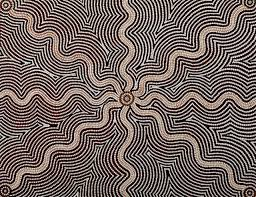
\includegraphics[width=3cm]{Population_study_design/Aboriginal_art2.jpg}

\includegraphics[width=3cm]{Population_study_design/Aboriginal_art3.jpg}

\includegraphics[width=3cm]{Population_study_design/Aboriginal_art4.jpg}

\includegraphics[width=3cm]{Population_study_design/Aboriginal_art5.jpg}
\end{tcolorbox}


\subsubsection{Impressionist art}

% Impressionist Art

\begin{tcolorbox}
Which one of the following examples of Impressionist art do you like the best?

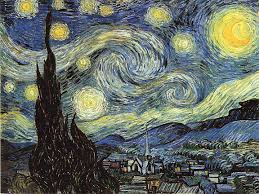
\includegraphics[width=3cm]{Population_study_design/Impressionist_art1.jpg}

\includegraphics[width=3cm]{Population_study_design/Impressionist_art2.jpg}

\includegraphics[width=3cm]{Population_study_design/Impressionist_art3.jpg}
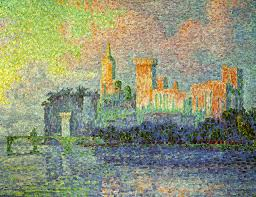
\includegraphics[width=3cm]{Population_study_design/Impressionist_art4.jpg}

\includegraphics[width=3cm]{Population_study_design/Impressionist_art5.jpg}
\end{tcolorbox}


\subsubsection{Sentences}

% Sentences

This domain consists of sentences that have been used in experiments of linguistic judgement.
They are, respectively sentences 7j, 7h, 7p, 7a and 7e in \citeasnoun{BardRobeSora96}.
Figure 1 of that paper shows acceptability scores for these and other sentences given by two individual linguists, an acceptability score aggregating the scores of four linguists and an acceptability score aggregating the scores of four ``naive respondents'', all undergraduate anatomy students.
There is broad, but not perfect, agreement in terms of order, and in the following list, they are in decreasing order of acceptability according to the measure aggregating the judgements of four linguists.

\begin{tcolorbox}
Which one of the following sentences do you find the most grammatically acceptable?

\begin{itemize}
	\setlength\itemsep{-5pt}
	\item Who did Bill buy the car to please?
	\item This is a book which reading would be fun.
	\item Where did Bill buy the car to drive?
	\item Which man do you wonder when to meet?
	\item With which pen do you wonder what to write?
\end{itemize}
\end{tcolorbox}


\subsubsection{Travel}

% Travel

The source is Tripadvisor.
These are the top five travel destinations, according to the results of an on-line contest where visitors to a Tripadvisor site could make pairwise choices between travel destinations.

\begin{tcolorbox}
\begin{quotation}
Which one of the following travel destinations would you most like to visit?
\end{quotation}

\begin{enumerate}
\item Marrakech, Morocco

\includegraphics[height=2.8cm]{Population_study_design/Travel1.jpg}

\item Istanbul, Turkey

\includegraphics[height=2.8cm]{Population_study_design/Travel2.jpg}

\item Hanoi, Vietnam

\includegraphics[height=2.8cm]{Population_study_design/Travel3.jpg}

\item Siem Reap, Cambodia

\includegraphics[height=2.8cm]{Population_study_design/Travel4.jpg}

\item Praque, Czech Republic

\includegraphics[height=2.8cm]{Population_study_design/Travel5.jpg}
\end{enumerate}	
\end{tcolorbox}


\subsubsection{Marijuana}

% Marijuana

This question elicits policy preferences.

\begin{tcolorbox}
Which one of the following marijuana policies would you choose?

\begin{itemize}
	\setlength\itemsep{-5pt}
	\item Possession by, and sales to adults are both legal; sales to minors are illegal.
	\item Possession by, and sales to adults are both illegal but neither is a criminal offense; sales to minors are a criminal offense.
	\item Possession is illegal but not criminal; all sales are a criminal offense.
	\item Possession and sales are criminal offenses, with a small number of medical exceptions.
	\item Possession and sales are criminal offenses, without exception.
\end{itemize}
\end{tcolorbox}


\subsection{Single attributes, not directly observed}

The five domains in this section contain choice objects with an objective rank order.

\subsubsection{Latitude}

% Latitude

The five cities of this domain have a latitude close to 50 degrees north.
In the following list, they are ordered from furthest north to furthest south.
According to Wikipedia, their latitudes are, respectively, $52\degree14^\prime N$, $51\degree30^\prime N$, $49\degree15^\prime N$, $48\degree51^\prime N$ and $47\degree36^\prime N$.
There are two potential asymmetric dominance effects, with Vancouver being fairly obviously north of Seattle and London being fairly obviously north of Paris.

\begin{tcolorbox}
Which one of the following cities do you think is furthest north?

\begin{itemize}
	\setlength\itemsep{-5pt}
	\item Warsaw, Poland
	\item London, United Kingdom
	\item Vancouver, Canada
	\item Paris, France
	\item Seattle, United States
\end{itemize}
\end{tcolorbox}


\subsubsection{Dots}

% Dots

This domain is a perception example.
The true numbers of points are, respectively, 320, 310, 300, 290 and 280.
It is much clearer that there are more points in the first panel than in the fifth, than that there are more points in the first than in the second.
The difference in the number of points is an obvious similarity measure here that might be expected to lead to similarity effects.
{}
\begin{tcolorbox}
Which one of the following boxes do you think has the greatest number of points?

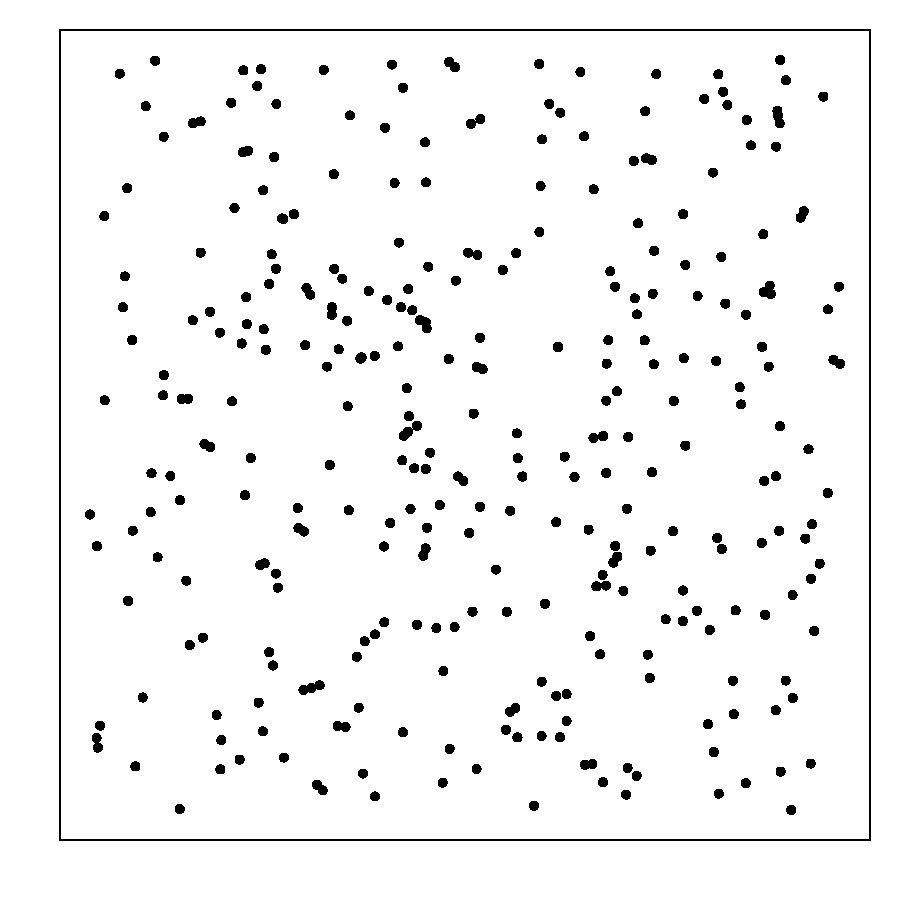
\includegraphics[height=3cm]{Population_study_design/Scatterplots1.pdf}
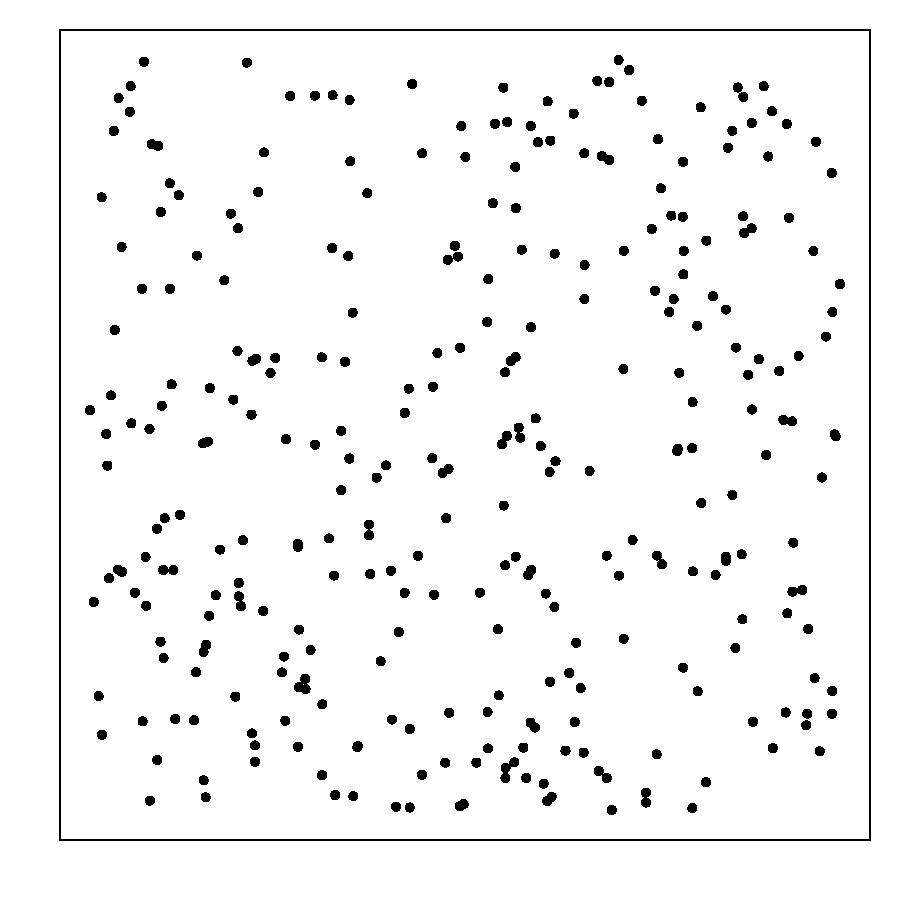
\includegraphics[height=3cm]{Population_study_design/Scatterplots2.pdf}
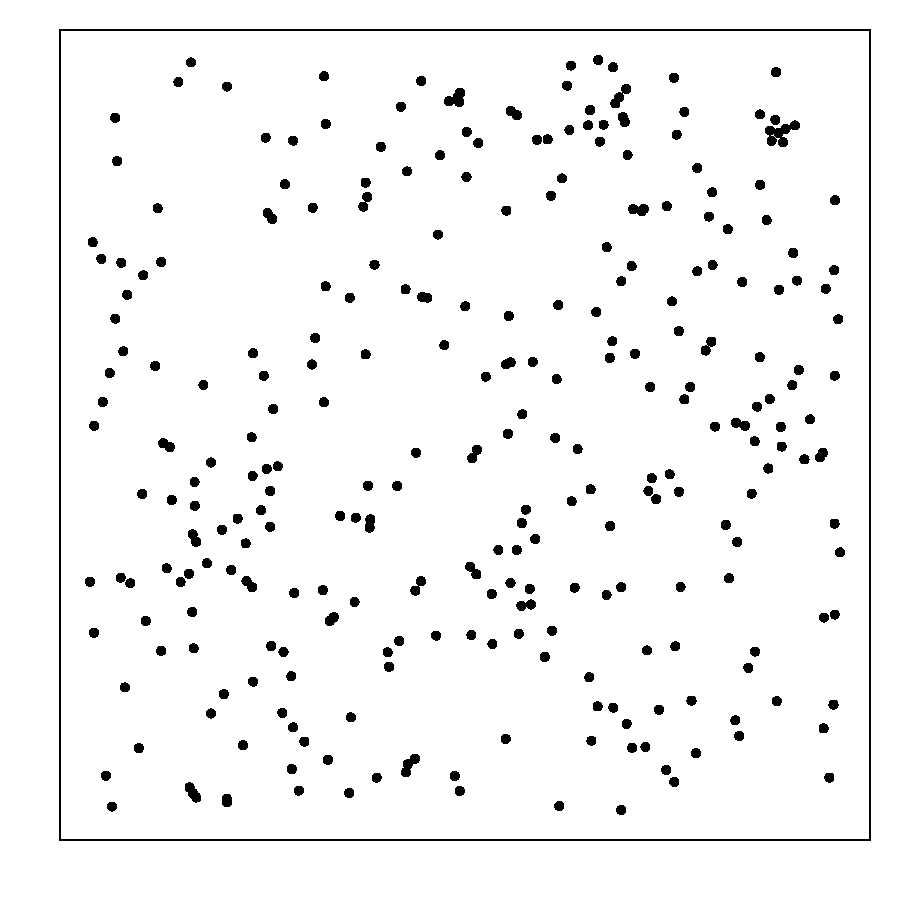
\includegraphics[height=3cm]{Population_study_design/Scatterplots3.pdf}
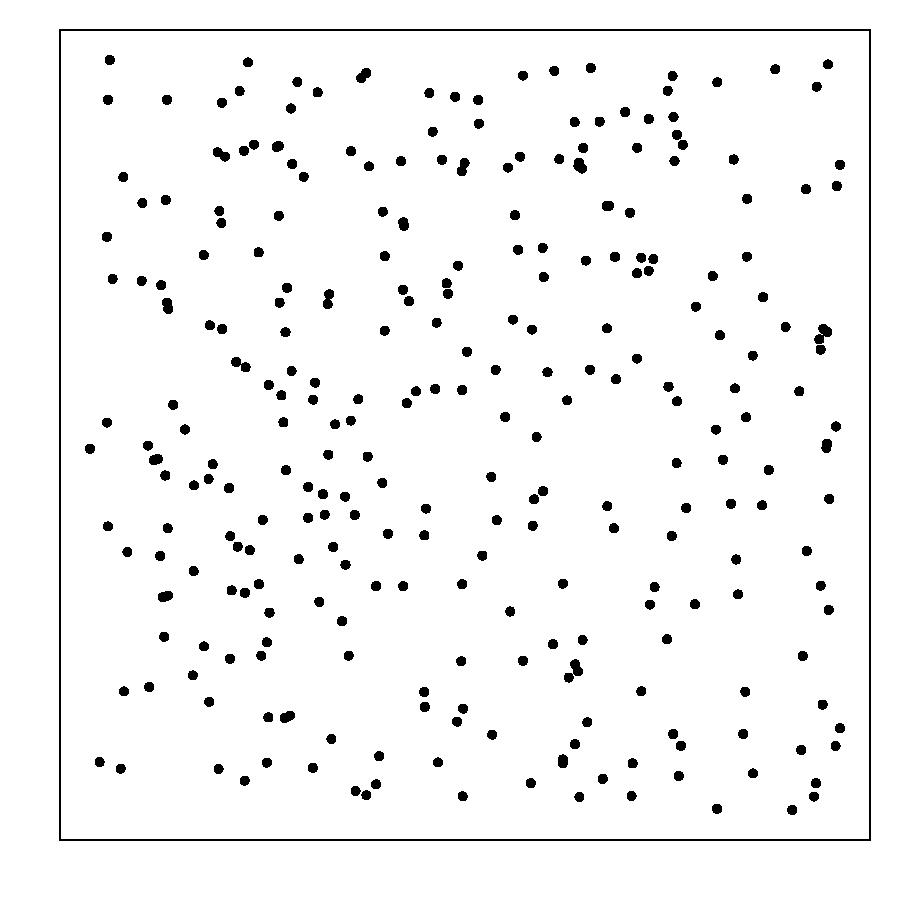
\includegraphics[height=3cm]{Population_study_design/Scatterplots4.pdf}
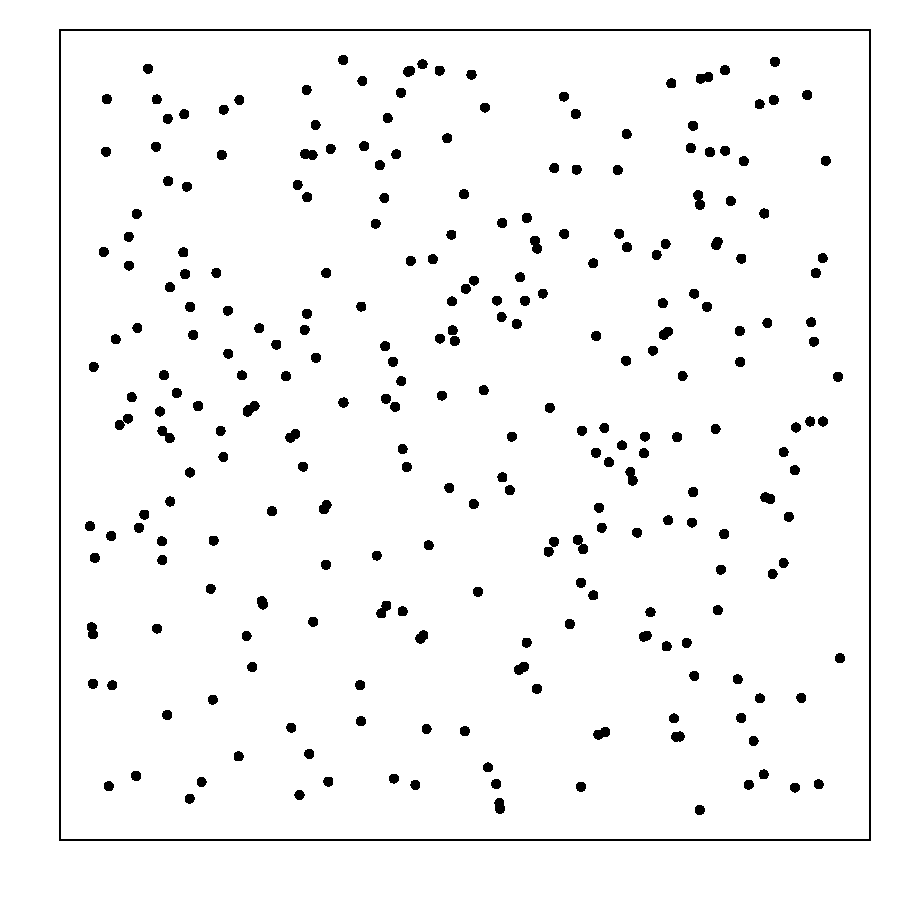
\includegraphics[height=3cm]{Population_study_design/Scatterplots5.pdf}
\end{tcolorbox}


\subsubsection{Triangles}

% Triangles

This domain is another perception example.
The true areas are, respectively, 16, 15, 15, 14 and 14 units.

\begin{tcolorbox}
	Which one of the following triangles do you think has the greatest area?

	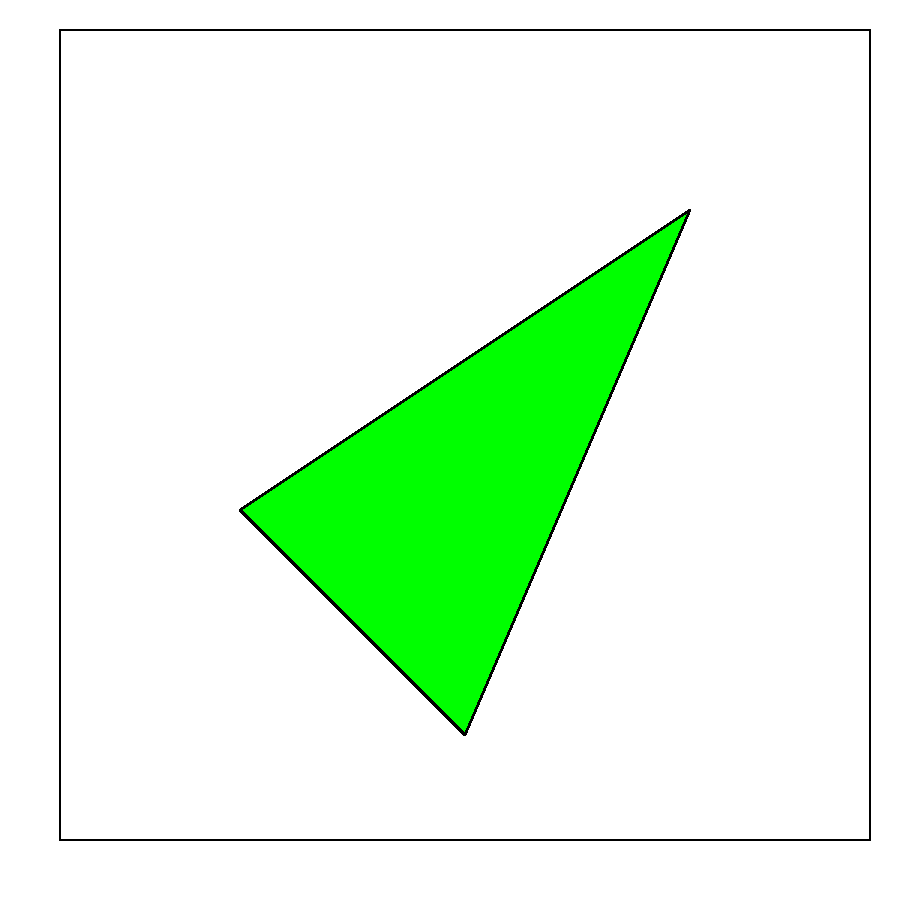
\includegraphics[height=3cm]{Population_study_design/Triangles3.pdf}
	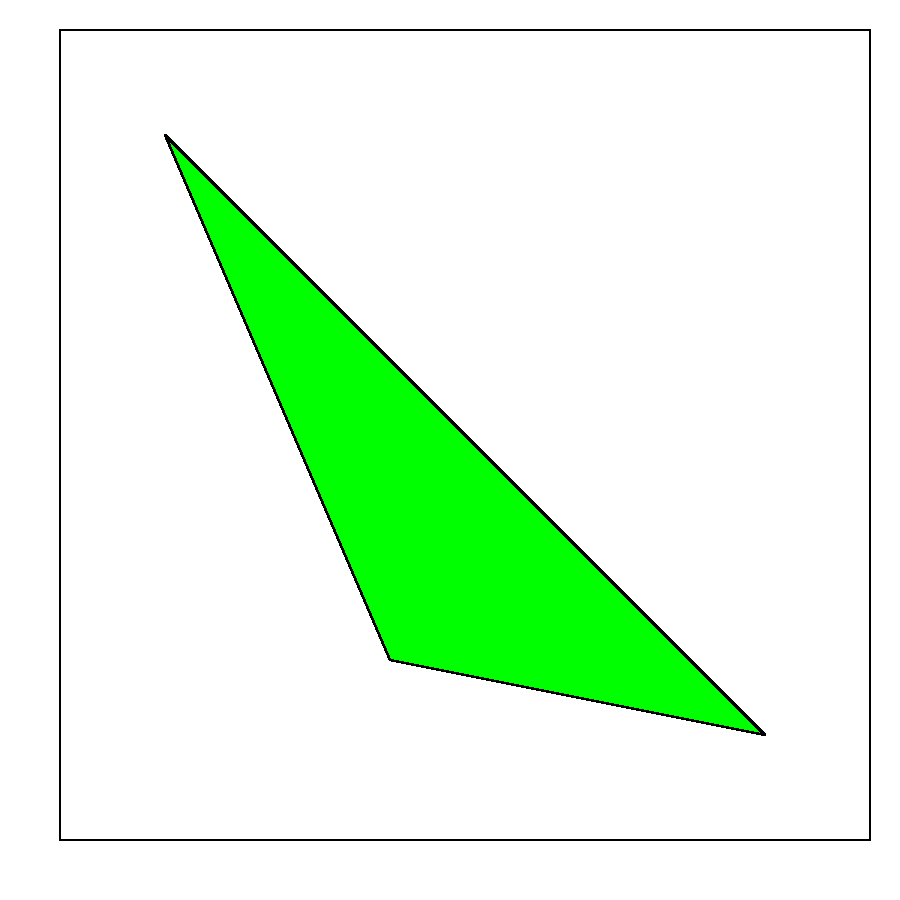
\includegraphics[height=3cm]{Population_study_design/Triangles1.pdf}
	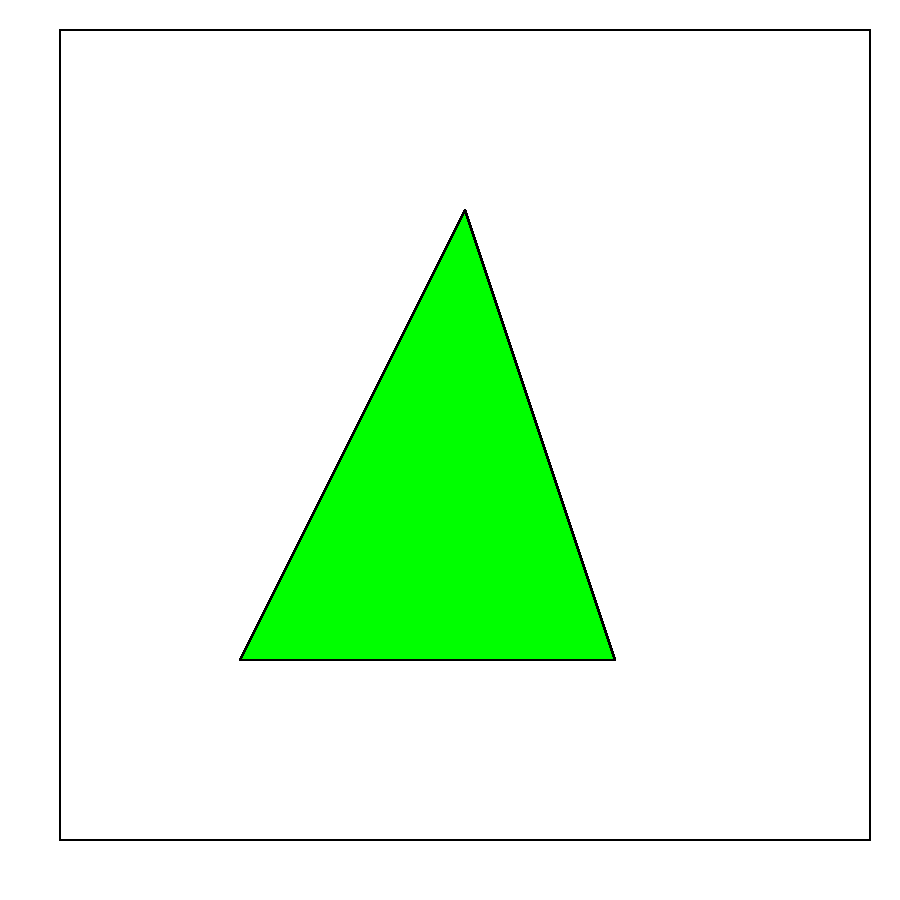
\includegraphics[height=3cm]{Population_study_design/Triangles2.pdf}
	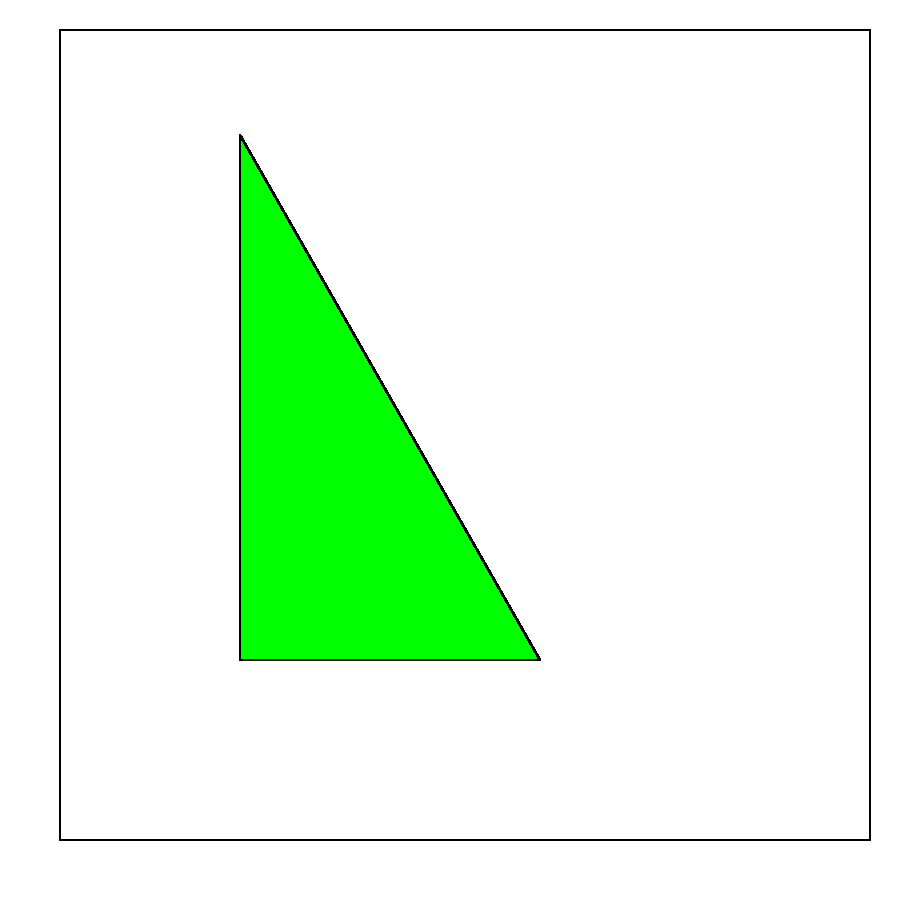
\includegraphics[height=3cm]{Population_study_design/Triangles4.pdf}
	
\includegraphics[height=3cm]{Population_study_design/Triangles5.pdf}	
\end{tcolorbox}


\subsubsection{Population}

% Population

These countries were ranked, respectively, 4th through 8th in terms of population in 2016, when
their populations, in millions, were 258, 206, 202, 186 and 156.

\begin{tcolorbox}
Which one of the following countries do you think has the largest population?

\begin{itemize}
	\setlength\itemsep{-5pt}
	\item Indonesia
	\item Brazil
	\item Pakistan
	\item Nigeria
	\item Bangladesh
\end{itemize}
\end{tcolorbox}


\subsubsection{Surface area}

% Surface area

These countries are ranked, respectively, 2nd through 6th in terms of surface area, including inland bodies of water.
In millions of square kilometres, those surface areas are 9.984, 9.573, 9.525, 8.516 and 7.692.

\begin{tcolorbox}
Which one of the following countries do you think has the greatest surface area, including inland bodies of water?
	
\begin{itemize}
	\setlength\itemsep{-5pt}
	\item Canada
	\item United States of America
	\item China
	\item Brazil
	\item Australia
\end{itemize}
\end{tcolorbox}


\subsection{Objects with two attributes}

Here we describe domains whose choice objects have exactly two real-valued attributes.
In all cases, the levels of these attributes are presented directly to the participant.
Figure \ref{f:CE} plots the five objects of each of these domains in attribute space, revealing potential conditions for context effects.

\begin{figure}
	\caption{Designs for context effects. Each panel plots the five objects of a domain in attribute space. The domains are, in row major order, Beer, Cars, Restaurants, Flights I, Delayed Choice, Phone Plans, Hotels}\label{f:CE}
	\centering
	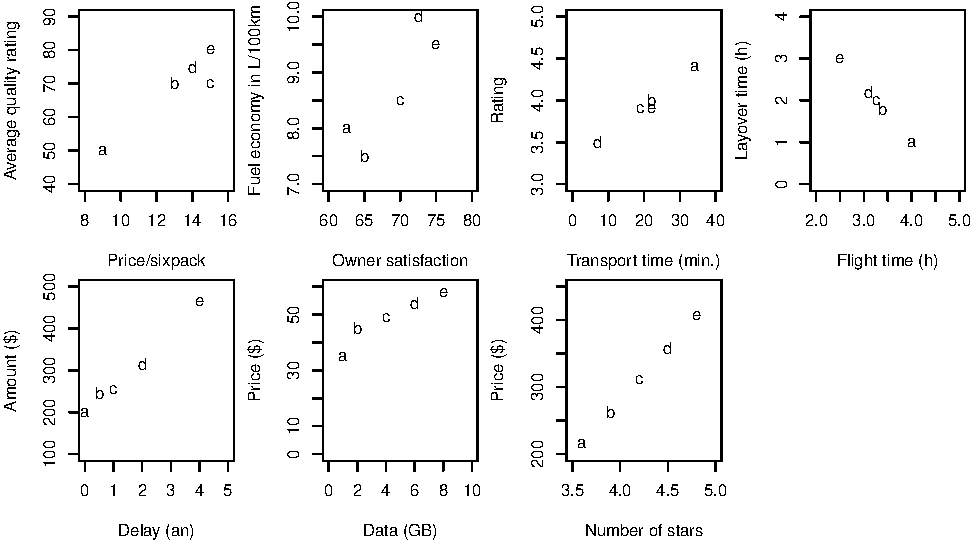
\includegraphics[width=15cm]{./Figures/design_patterns.pdf}
\end{figure}

Table \ref{t:CE} shows, for the first four of these domains, dominance, similarity and betweenness relations that we might expect to generate context effects.
Following usual practice, we exclude similarity relations for two objects in which there is also a dominance relation between the two; and betweenness relations among three objects when two of them are similar and the third is not similar to either of the first two.

\begin{table}
	\centering
	\begin{tabular}{cccc}
		Domain & Dominance & Similarity w/o dominance & Betweenness w/o similarity \\
		\hline
		Beer
		& $e>c$, $b>c$, $d>c$ & $b \sim d$, $d \sim e$, $b \sim e$
		& $a|b|e$ \\
		Cars
		& $a>d$, $b>e$ & & $a|c|b$, $a|c|e$, $a|c|b$, $d|c|e$ \\
		Restaurants
		& $b>e$, $c>e$ & $b \sim c$ & $a|b|d$, $a|c|d$, $a|e|d$ \\
		Flights I 
		& & $b \sim c$, $c \sim d$, $b \sim d$ & $a|b|e$, $a|c|e$, $a|d|e$ \\
		\hline
	\end{tabular}\caption{Relations of dominance, similarity and betweenness in two-attribute domains}\label{t:CE}
\end{table}

\subsubsection{Beer}

% Beer

This domain is from an experiment reported in \citeasnoun{HubePaynPuto82} used to illustrate an asymmetric dominance effect.
The prices are multiplied by 5 and we added choice objects d and e to allow for two more asymmetric dominance effects and two similarity effects.
The first panel of Figure \ref{f:CE} show the choice objects in attribute space.
Table \ref{t:CE} shows the relations of dominance, similarity and betweenness among objects associated with context effects.
The most commonly used domains to illustrate the attraction effect involve Beer, Cars, Apartments, Computers, Restaurants and Televisions.

\begin{tcolorbox}
Below you will find three brands of beer.
You know only the price per sixpack and the average quality ratings made by respondents in a blind taste test.
Given that you had to choose one brand to buy on this information alone, which one would you choose?

\begin{tabular}{cc}
\hline
Price/sixpack & Average quality rating (100 = Best; 0 = Worst) \\ 
\hline
\$9.00 & 50 \\ 
\$13.00 & 70 \\ 
\$15.00 & 70 \\ 
\$14.00 & 75 \\ 
\$15.00 & 80 \\ \hline
\end{tabular}
\end{tcolorbox}


\subsubsection{Cars}

% Cars

This domain is based on an experiment from \citeasnoun{WedePett96}.
There are two experiments involving cars in that article, the experiment in question is  numbered 18 in the appendix to that paper.
Objects below have the same attributes as in that experiment and a similar range of levels.
We adapted the objects to allow for compromise effects.
The second panel of Figure \ref{f:CE} shows the choice objects in attribute space.
Table \ref{f:CE} shows the relations of dominance, similarity and betweenness among objects associated with context effects.

\begin{tcolorbox}
Which one of the following cars would you choose to drive, all other features
begin equal? Ride quality is a on a scale of 0 to 100.

\begin{tabular}{cc}
\hline
Ride quality & Miles per gallon \\ \hline
60 & 30 \\ 
80 & 24 \\ 
70 & 27 \\ 
55 & 28 \\ 
75 & 22 \\ \hline
\end{tabular}
\end{tcolorbox}


\subsubsection{Restaurants}

% Restaurants

This domain is based on another experiment in \citeasnoun{WedePett96}, numbered 19 in the appendix to that paper.
The third panel of Figure \ref{f:CE} shows the choice objects in attribute space.
Table \ref{t:CE} shows the relations of dominance, similarity and betweenness among objects associated with context effects.

\begin{tcolorbox}
Which one of the following restaurants would you choose for your next restaurant meal, based on transportation time (in minutes) and average customer ratings (from
1 to 5).
	
\begin{tabular}{cc}
\hline
Transportation time & Rating \\ \hline
34 & 4.4 \\ 
22 & 4.0 \\ 
19 & 3.9 \\ 
7 & 3.5 \\ 
22 & 3.9 \\ \hline
\end{tabular}
\end{tcolorbox}


\subsubsection{Layovers}

% Layovers

The fourth panel of Figure \ref{f:CE} shows the choice objects in attribute space.
Table \ref{t:CE} shows the relations of dominance, similarity and betweenness among objects associated with context effects.

\begin{tcolorbox}
Which one of the following flight itineraries would you choose?
All involve two flights, with one layover between them.

\begin{tabular}{ccc}
\hline
Total inflight time & Layover time & Total itinerary time \\ \hline
4:00 & 1:00 & 5:00 \\ 
3:24 & 1:48 & 5:12 \\ 
3:15 & 2:00 & 5:15 \\ 
3:06 & 2:12 & 5:18 \\ 
2:30 & 3:00 & 5:30 \\ \hline
\end{tabular}
\end{tcolorbox}


\subsubsection{Delayed Choice}

% Delayed choice

This domain is loosely based on an experiment by \citeasnoun{BenzRapoYagi89}, in which respondents are asked to assign present values equivalent to the receipt of \$200 at time horizons of 0.5, 1, 2 and 4 years.
Based on implied discount factors at various terms, we constructed five choice objects designed to have approximately the same present value equivalent.

\begin{tcolorbox}
Which one of the following would you choose?

\begin{itemize}
	\setlength\itemsep{-5pt}
	\item \$200 credited to your bank account immediately.
	\item \$245 credited to your bank account in six months.
	\item \$255 credited to your bank account in one year.
	\item \$315 credited to your bank account in two years.
	\item \$465 credited to your bank account in four years.
\end{itemize}
\end{tcolorbox}


\subsubsection{Phone plans}

% Phone plans

The source for this domain is the website of Fido Mobile, with rates quoted on March 1, 2017 in Canadian dollars.

\begin{tcolorbox}
Of the following cell phone plans, which one would you choose? In all cases, unlimited calling, text picture and video messages to Canadian and international mobile numbers are included. Excess data usage is billed at \$10 per 500 MB.

\begin{itemize}
	\setlength\itemsep{-5pt}
	\item 1 GB data per month, \$35 per month.
	\item 2 GB data per month, \$45 per month.
	\item 4 GB data per month, \$49 per month.
	\item 6 GB data per month, \$54 per month.
	\item 8 GB data per month, \$58 per month.
\end{itemize}
\end{tcolorbox}


\subsubsection{Hotel rooms}

% Hotel rooms

Using Expedia results, I did a linear regression of price per night on a constant and the Expedia rating, in numbers of stars, for a sample of available hotels.
The five levels of numbers of stars correspond roughly to the mean, plus and minus one sample standard deviation and plus and minus two standard deviations.
Prices are approximately equal to fitted values in the linear regression.

\begin{tcolorbox}
Suppose you are staying over two nights in New York city.
Which one of the following hotels would you choose, based on customer ratings and price per night?	

\begin{itemize}
	\setlength\itemsep{-5pt}
	\item 3.6/5 stars, \$215 per night
	\item 3.9/5 stars, \$263 per night
	\item 4.2/5 stars, \$311 per night
	\item 4.5/5 stars, \$358 per night
	\item 4.8/5 stars, \$406 per night
\end{itemize}
\end{tcolorbox}


\subsection{Objects with multiple attributes}

\subsubsection{Flight itineraries}

% Flight itineraries

This domain illustrates three-way tradeoffs.
The points form a constellation in the simplex that resembles the pattern of points on the ``five'' side of a die.

\begin{tcolorbox}
Which one of the following flight itineraries would you choose? All involve two
flights and have a total duration of six hours.

\begin{tabular}{ccc}
\hline
	1st flight & Layover & 2nd flight \\ \hline
	1:30 & 1:15 & 3:15 \\ 
	3:15 & 1:15 & 1:30 \\ 
	2:15 & 1:30 & 2:15 \\ 
	1:30 & 1:45 & 2:45 \\ 
	2:45 & 1:45 & 1:30 \\ \hline
\end{tabular}
\end{tcolorbox}


\subsubsection{Televisions}

% Televisions

The source for this domain is the website of Best Buy Canada, with prices in Canadian dollars.

\begin{tcolorbox}
Which one of the following televisions would you choose to buy if you
were in the market for a television? All are LED televisions. Resolution
refers to number of horizontal lines. Smart indicates internet connectivity.

\begin{tabular}{ccccccc}
\hline
Brand & Resolution & Smart & Price (\$) & Screen Size (inches) &  \\ \hline
Sharp & 1080 & Yes & 309 & 32 &  \\ 
Insignia & 720 & No & 209 & 32 &  \\ 
Sony & 720 & Yes & 439 & 32 &  \\ 
Samsung & 1080 & Yes & 459 & 40 &  \\ 
Toshiba & 1080 & No & 409 & 43 &  \\
\hline
\end{tabular}
\end{tcolorbox}


\subsubsection{Coffee}

% Coffee

The source for this domain is the website \texttt{buycoffeecanada.com}, with prices in Canadian dollars.

\begin{tcolorbox}
You need to buy 16oz of ground coffee for a brunch with friends.
Which one of the following ground coffees would you choose?

\begin{tabular}{rcl}
\hline
Price & Fair Trade & Name: Description \\
\hline
18.71 & Yes & Ethiopian Yirgacheffe: vibrant and intensely aromatic, fruity \\
9.99 & No & Colombian Supremo: mellow cup, complex aromas and rich flavours \\
13.72 & Yes & Colombian Organic: medium body, fragrant aroma and mild acidity \\
12.35 & No & Tanzania Peaberry: full bodied coffee, chocolatey aroma, wine-like finish \\
13.46 & No & Sumatra Mandheling: exotic, earthy, bright with low acidity \\
\hline
\end{tabular}
\end{tcolorbox}


\subsubsection{Charity}

% Charity

The charities in this domain are real charities.
The first two are relatively innocuous in the sense that most people support the goals of both.
However, the Canadian Cancer Society attracts much more financial support than Arthritis Research Canada and we might expect that most people would prefer a marginal dollar going to the former.
The two other charities have goals that are nearly opposite and elicit strong emotions (of different kinds) from some.

\begin{tcolorbox}
Suppose someone was donating a total of 100 dollars to a combination of charities,
on your behalf.
Which one of the following divisions of the 100 dollars would you choose?

\begin{tabular}{p{35mm}|p{35mm}|p{35mm}|p{35mm}}
\hline
Arthritis Research Canada &
Canadian Cancer Society &
Canadian Coalition for Firearm Rights &
Coalition for Gun Control \\
\hline
90 & 10 & 0 & 0 \\
35 & 60 & 5 & 0 \\
35 & 60 & 0 & 5 \\
10 & 80 & 10 & 0 \\
10 & 80 & 0 & 10 \\
\hline
\end{tabular}
\end{tcolorbox}


\bibliographystyle{agsm}
\bibliography{bibliography}

\end{document}